\documentclass[a4paper, 11pt]{scrartcl}
\usepackage[utf8]{inputenc}
\usepackage[top = 2.5cm, bottom = 2cm, left = 2.5cm, right = 2.5cm]{geometry}
\usepackage[onehalfspacing]{setspace}
\usepackage{mathtools}
\usepackage{fontspec}
\usepackage{graphicx}
\usepackage{rotating}
\usepackage[english]{babel}
\usepackage{enumerate}
\usepackage{tabularx}
\usepackage{booktabs}
\usepackage{hyperref}
\hypersetup{colorlinks = true, linkcolor = black, citecolor = blue, urlcolor = blue}
\usepackage{csquotes}
\usepackage[backend = biber, style = apa]{biblatex}
\addbibresource{../iris_literature.bib}

\title{IRIS model validation: Lessons learned}
\author{}
\date{\today}

\begin{document}
\maketitle
\tableofcontents

\newpage
\section{Motivation}
The IRIS model was validated with observation data from a sampling site near Regensburg. The aim of the model validation was to check how well the simulated model results match
with observed data. This includes the analysis of the influence of parameters for which we either found no clear values in the literature (e.g.\ for the activation rate) or
which change from year to year but are needed for initialisation such as the initial number of larvae or nymphs. In this context, we have also analysed the beech mast which
modulates the initial number of larvae which in turn affects the second peak of questing nymphs in a given year. For this purpose, we have performed sensitivity analyses over a
range of plausible values for these parameters and quantified the matching of the simulation results with the observed data from the sampling site. Here, we present the results
of this validation.


\section{Validation data}
For the validation we used a data set with monthly observations of nymphal ticks per $100 m^2$ of a 10-year period from a sampling site in Haselmühl where
\textit{Ixodes ricinus} ticks were collected using the flagging method~\parencite{Brugger.2017}. The time series with data between 2009 and 2018 was provided by
Gerhard Dobler\footnote{Bundeswehr Institute of Microbiology, Neuherbergstraße 11, 80937 Munich, Germany} via our cooperation partner Katharina
Brugger\footnote{Institute for Veterinary Public Health, University of Veterinary Medicine Vienna, Veterinärplatz 1, 1210 Vienna, Austria}. The observation data was also
used for model validation by~\textcite{Brugger.2017, Brugger.2018}.


\section{Evaluation criteria}
We use the root mean square error (RMSE) to quantify the differences of the simulated from the observed monthly nymphal densities. It was calculated for each of the 10 years of
the available validation data using the following formula:

\begin{equation}\label{eq:rmse}
RMSE_{year} = \sqrt{ \frac{1}{n} \sum_{i=1}^n (V_{sim}^i - V_{obs}^i)}
\end{equation}

with total number of monthly observations $n$, observed values $V_{obs}$ and simulated values $V_{sim}$ of a given year. A perfect fit corresponds to an RMSE value of 0, i.e.\
simulated and observed data match exactly. The higher an RMSE value the poorer is the matching. Months with missing data (NA-values) were not taken into account when
calculating the RMSE of a given year.

In order to evaluate the entire 10-year validation period, the annual RMSE values were added up and a total root mean square error $RMSE_{total}$ was calculated, hence
\begin{equation}\label{eq:total_rmse}
RMSE_{total} = \sum_{year=2009}^{2018} RMSE_{year}
\end{equation}


\section{Sensitivity Analyses}
We conducted sensitivity analyses to analyse the influence of the (1) initial number of larvae, (2) the initial number of nymphs and (3) the activation rate of the activity sub
model.

The initial number of larvae and nymphs at the beginning of a simulation run has an influence on the number of active nymphs throughout the year including the height of the
abundance peaks. Since we were interested in how the initial number of ticks controls the abundance peaks and since we didn't know the real initial values at the beginning of a
simulation, we were interested in the influence of these parameters. In this context, we analysed the influence of the beech mast process of our model. In
particular we analysed out whether the beech mast improves the matching of the model output with the real data\footnote{For details regarding the beech mast
see the ODD protocol of the IRIS model.}. Therefore, the sensitivity analyses were carried out with both the beech mast activated and deactivated.

The activation rate $r$ is an important model parameter. It is responsible for controlling the number of questing and inactive ticks in each time step. When microclimatic
conditions are suitable for questing, the number of questing ticks increases with a specific activation rate and the number of inactive ticks is reduced accordingly (and vice
versa)\footnote{For details regarding the activity sub model see the ODD protocol of the IRIS model.}. We estimated the activation rate through systematic variation within the
presented sensitivity analyses. There is no value for this parameter available in the literature because it is an artefact of our cohort-based approach and
therefore from a biological point of view an unreasonable parameter for which no measurements exists. We have carried out five sensitivity analyses:

\begin{enumerate}
\item[] \textbf{S1:} Equal number of larvae and nymphs, with beech mast activated
\item[] \textbf{S2:} Equal number of larvae and nymphs, with beech mast deactivated
\item[] \textbf{S3:} Larvae and nymphs individual variation, with beech mast activated
\item[] \textbf{S4:} Larvae and nymphs individual variation, with beech mast deactivated
\item[] \textbf{S5:} Higher share of initial number of Larvae, with beech mast activated
\end{enumerate}

In the first two sensitivity analyses (S1, S2), the initial number of larvae and nymphs was kept equal when varying these parameters within the sensitivity analysis (i.e.\ in
the for-loop). If, however, the beech mast model process was activated, the initial number of larvae was adjusted at the beginning of the simulation run, resulting in the actual
starting values being different. In the subsequent analyses (S3, S4), the number of larvae and nymphs was varied individually. At the beginning of a simulation run, the initial
numbers of larvae and nymphs could therefore differ considerably. An additional analysis (S5) was carried out to test the effect of the initial number of larvae being
significantly greater than the initial number of nymphs. The results are presented in the following sections.


\subsection{S1: Equal number of larvae and nymphs, with beech mast activated}
In this sensitivity analysis we varied the initial number of larvae and nymphs and the activation rate $r$ in a first step in the following way:

\begin{enumerate}
\item The initial number of nymphs was varied \underline{from} \textbf{2} \underline{to} \textbf{1000} with a \underline{step size} of \textbf{2}.
\item The initial number of larvae was set to the initial number of nymphs.
\item The activation rate was varied \underline{from} \textbf{0.001} \underline{to} \textbf{0.030} with a \underline{step size} of \textbf{0.001}.
\end{enumerate}

Figure~\ref{fig:initial_ticks_with_beech_error_v1} shows the 3D scatterplots for all 10 validation years of the sensitivity analysis, i.e.\ the parameter variation of initial
larvae and nymphs (x-axis, labeled as \textit{ticks}) and activation rate (y-axis) and the RMSE value as evaluation criterion on the z-axis. It can be seen that the minimum RMSE
values for each year form a narrow band inside the three-dimensional parameter valley (indicated by the red color). The band stretches horizontally along the y-axis in a
confined area for initial ticks, but also makes a slight curve toward higher initial ticks in many cases, i.e.\ for the combination of small activation rate ($r < 5$) and large
number of initial ticks. Combinations of a high activation rate ($r > 20$) and a high number of initial ticks (greater than 500) corresponds to high RMSE values in
most cases. In all of the 10 validation years, there is no clearly identifiable minimum. Different parameter combinations lead to RMSE values that are all at a similarly low
level.

\begin{figure}[h!]
\centering
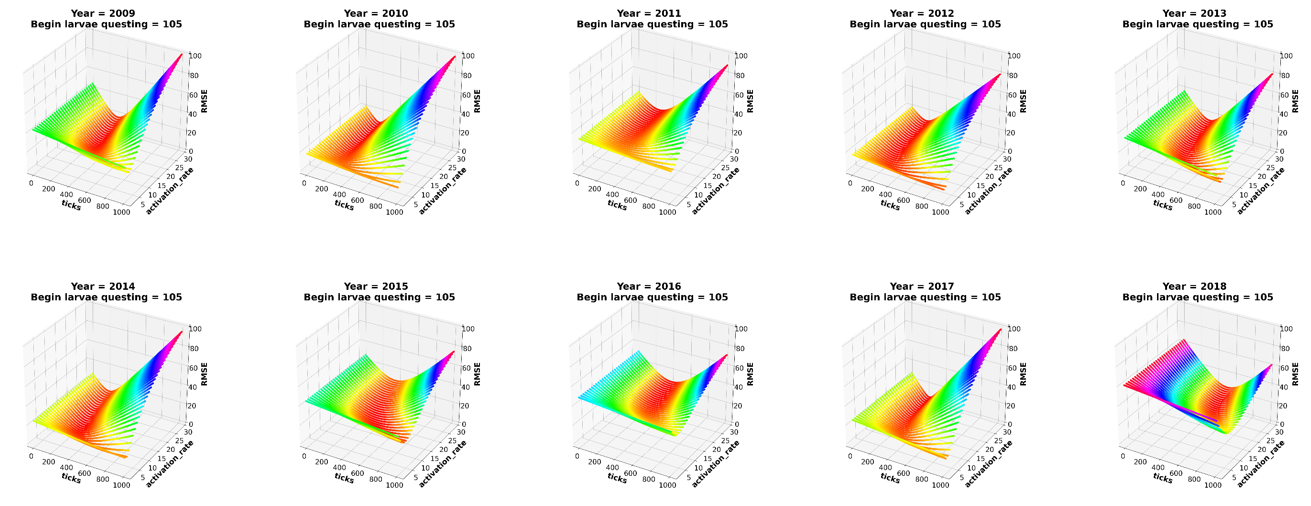
\includegraphics[width=\linewidth]{figures/initial_ticks_with_beech_error_v1}
\caption{3D scatterplots of \textbf{sensitivity analysis S1} for all 10 validation years (2009 - 2018). Each of the plots is contrasting the initial number of larvae and nymphs
(labeled as \textit{ticks}) on the x-axis, the activation rate on the y-axis and the RMSE on the z-axis. The colour indicates how large the RMSE value is. Shades of
red represent low RMSE values and shades of yellow, green and purple represent higher RMSE values.}
\label{fig:initial_ticks_with_beech_error_v1}
\end{figure}

To further narrow the range of parameters that lead to minimum RMSE values we decreased the step size of the sensitivity analysis from 2 to 1 with regard to the initial number of
larvae and nymphs and by decreasing the range of the activation rate in a second step. This sensitivity analysis was carried out in the the following way:

\begin{enumerate}
\item The initial number of nymphs was varied \underline{from} \textbf{1} \underline{to} \textbf{800} with a \underline{step size} of \textbf{1}.
\item The initial number of larvae was set to the initial number of nymphs.
\item The activation rate was varied \underline{from} \textbf{0.016} \underline{to} \textbf{0.022} with a \underline{step size} of \textbf{0.001}.
\end{enumerate}

In this sensitivity analysis it can be seen that the minimum values for each year are now located on a narrow band of initial ticks (see
Figure~\ref{fig:initial_ticks_with_beech_error}). Larger or smaller initial tick values lead to an increase of the RMSE value. Here, it can also be seen that the activation rate
does not clearly affect the RMSE. It should be noted, however, that the parameter range of the activation rate was chosen to be significantly smaller.

\begin{figure}[h!]
\centering
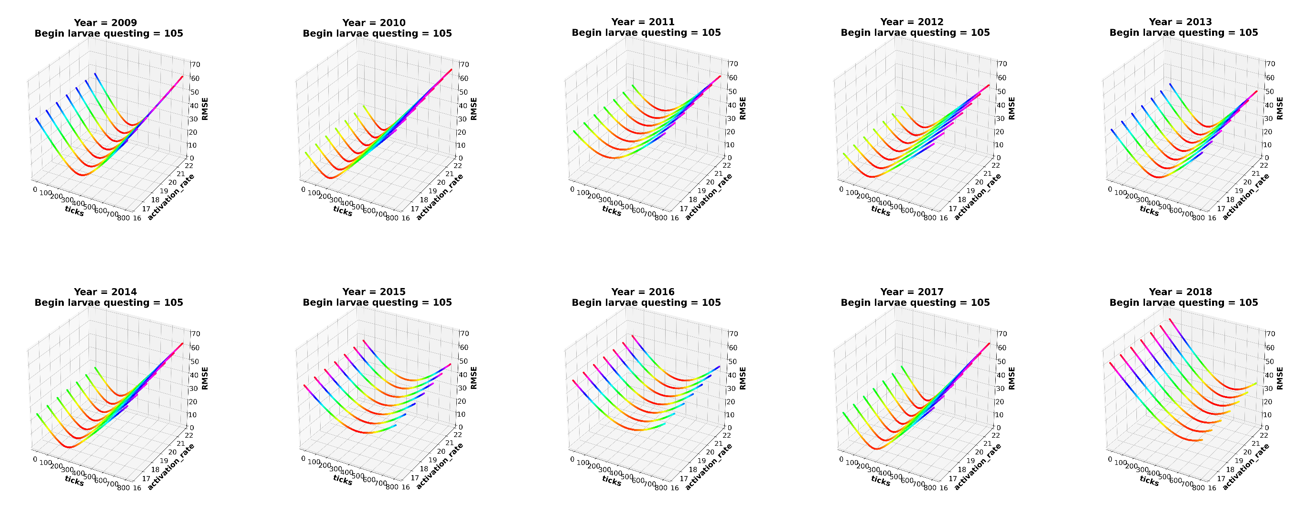
\includegraphics[width=\linewidth]{figures/initial_ticks_with_beech_error}
\caption{3D scatterplots of \textbf{sensitivity analysis S1} for all 10 validation years (2009 - 2018). Each of the plots is contrasting the initial number of larvae and nymphs
(labeled as \textit{ticks}) on the x-axis, the activation rate on the y-axis and the RMSE on the z-axis. The colour indicates how large the RMSE value is. Shades of red
represent low RMSE values and shades of yellow, green and purple represent higher RMSE values.}
\label{fig:initial_ticks_with_beech_error}
\end{figure}

In a further step, we calculated the activation rate that minimizes the total RMSE over all years. This is based on the assumption that from a biological point of view the
activation rate does not vary from year to year, but is the same across all years. For this sensitivity analysis we found the optimal activation rate to be $r_{opt} = 0.02$.

With this optimal activation rate, we took the corresponding initial number of ticks for each year, which minimises the RMSE and plotted the simulated monthly nymph densities
together with the monthly observation data to compare them also qualitatively (see Figure~\ref{fig:initial_ticks_with_beech}). This gives an overview of how the IRIS model
has captured the individual months of a given year. It can be seen very clearly that the first abundance peak matches the observation data qualitatively well in almost all years.
There are stronger deviations in 2011 (March is substantially underestimated), 2013 (April is substantially underestimated, May is substantially overestimated), 2014 (March is
substantially overestimated), 2016 (March is substantially underestimated) and 2018 (March is substantially overestimated, May is substantially underestimated). The second half
of a given year is not always captured well by the model. In particular, the observed second tick abundance peak is not well captured in many years. In some years a peak is
modelled although it does not actually exist (2009, 2011, 2016, 2018). In 2012, an abundance peak is not modelled even though it actually exists. In 2015, a very strong activity
peak is barely captured. The years 2010, 2012, 2014 and 2017 are captured relatively well by the model and have the lowest RMSE values ($\leq 8.37$) compared to the other years.
The sum of the RMSE values of the 10-year period is $RMSE_{total} = 147.85$.

\begin{figure}[h!]
\centering
\begin{minipage}[c]{0.40\linewidth}
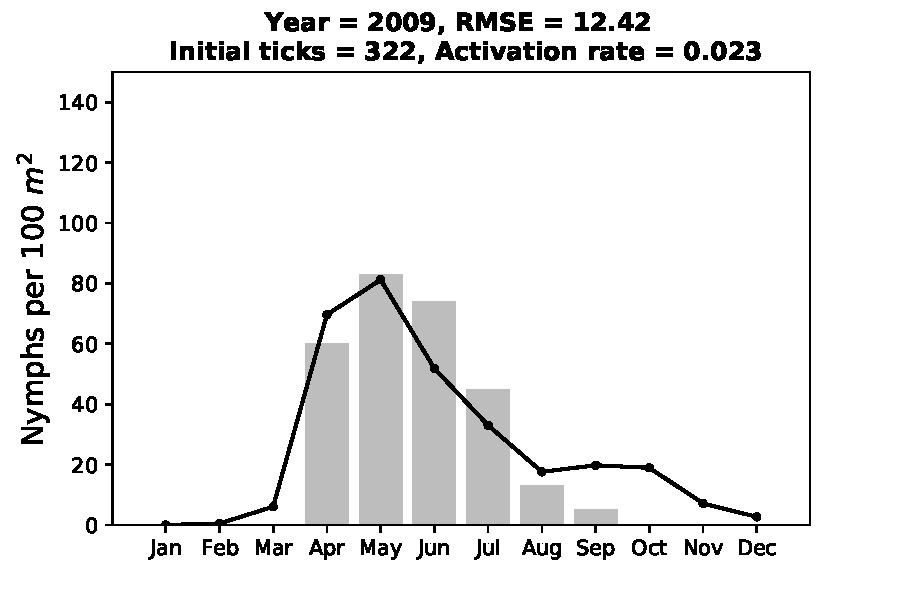
\includegraphics[width=\linewidth]{figures/s1/s1_2009}
\end{minipage}
\begin{minipage}[c]{0.40\linewidth}
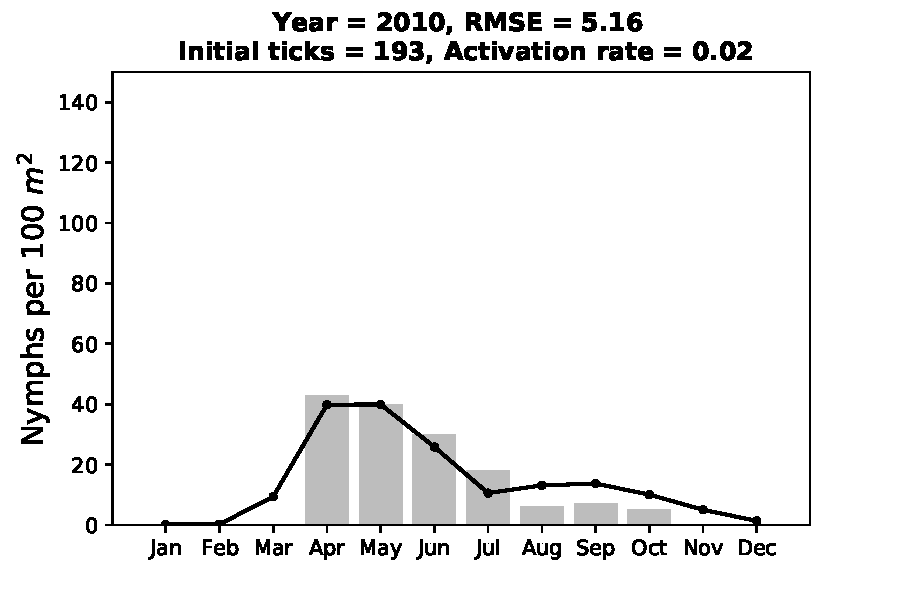
\includegraphics[width=\linewidth]{figures/s1/s1_2010}
\end{minipage}
\begin{minipage}[c]{0.40\linewidth}
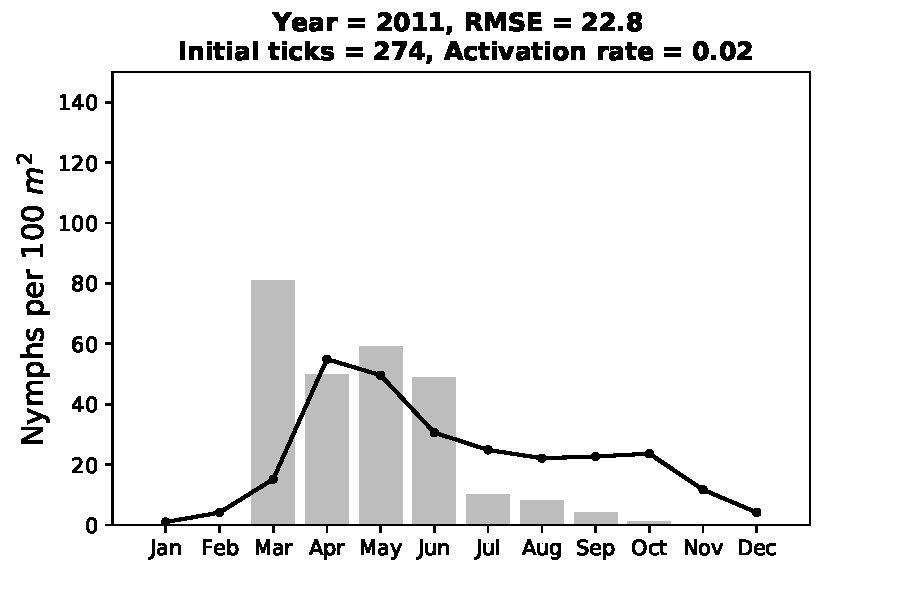
\includegraphics[width=\linewidth]{figures/s1/s1_2011}
\end{minipage}
\begin{minipage}[c]{0.40\linewidth}
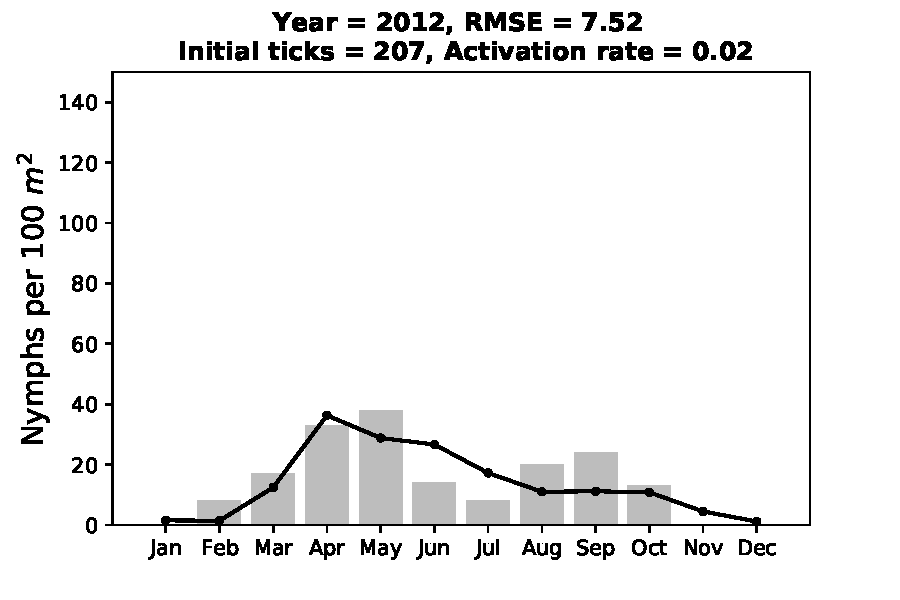
\includegraphics[width=\linewidth]{figures/s1/s1_2012}
\end{minipage}
\begin{minipage}[c]{0.40\linewidth}
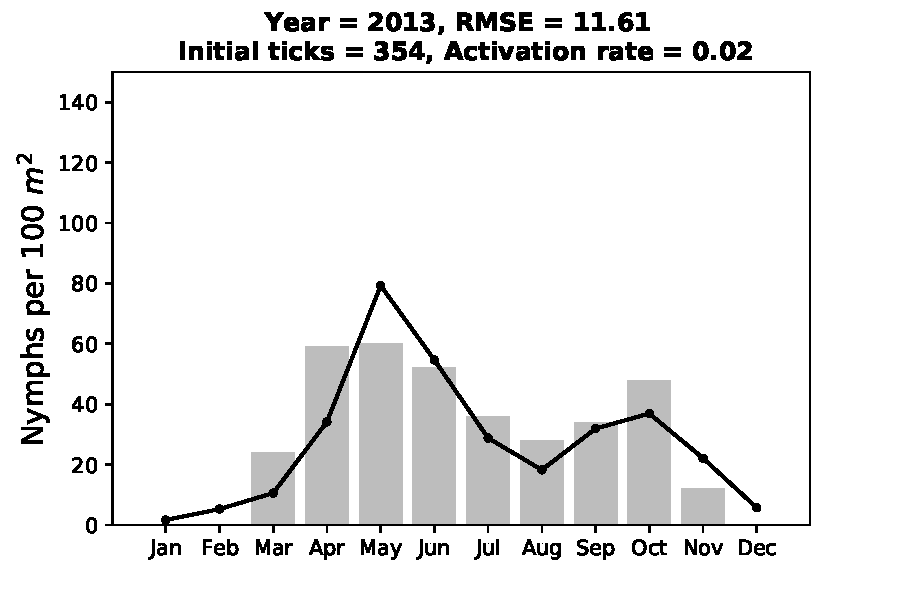
\includegraphics[width=\linewidth]{figures/s1/s1_2013}
\end{minipage}
\begin{minipage}[c]{0.40\linewidth}
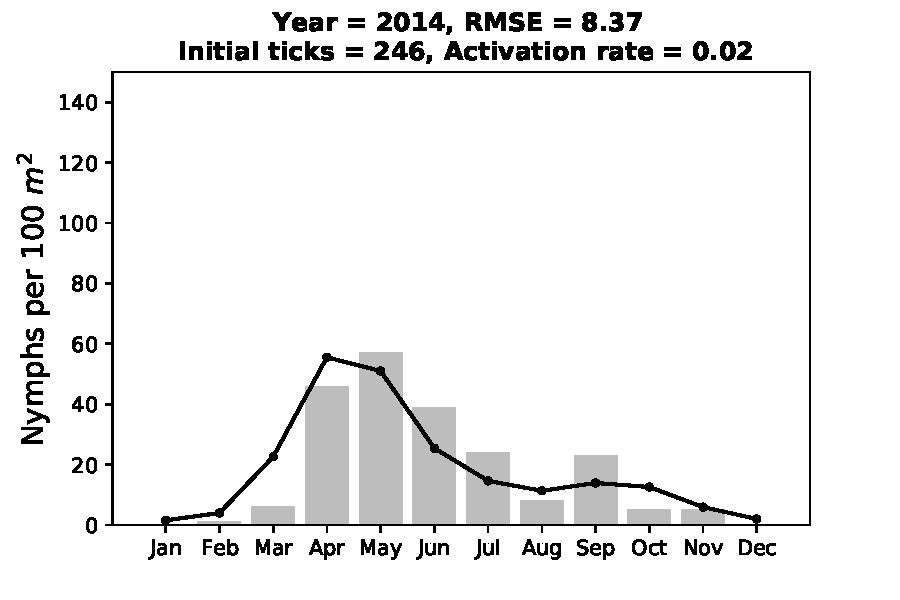
\includegraphics[width=\linewidth]{figures/s1/s1_2014}
\end{minipage}
\begin{minipage}[c]{0.40\linewidth}
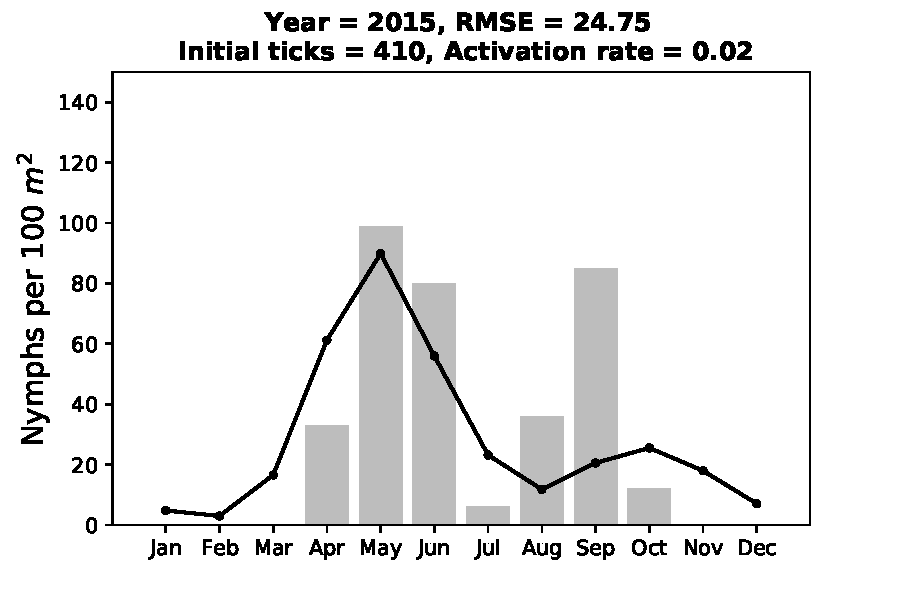
\includegraphics[width=\linewidth]{figures/s1/s1_2015}
\end{minipage}
\begin{minipage}[c]{0.40\linewidth}
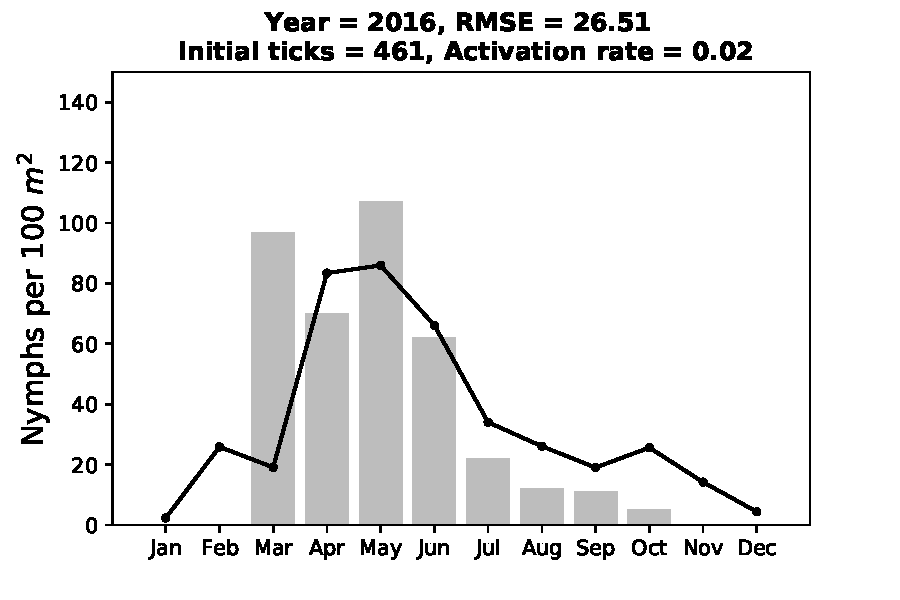
\includegraphics[width=\linewidth]{figures/s1/s1_2016}
\end{minipage}
\begin{minipage}[c]{0.40\linewidth}
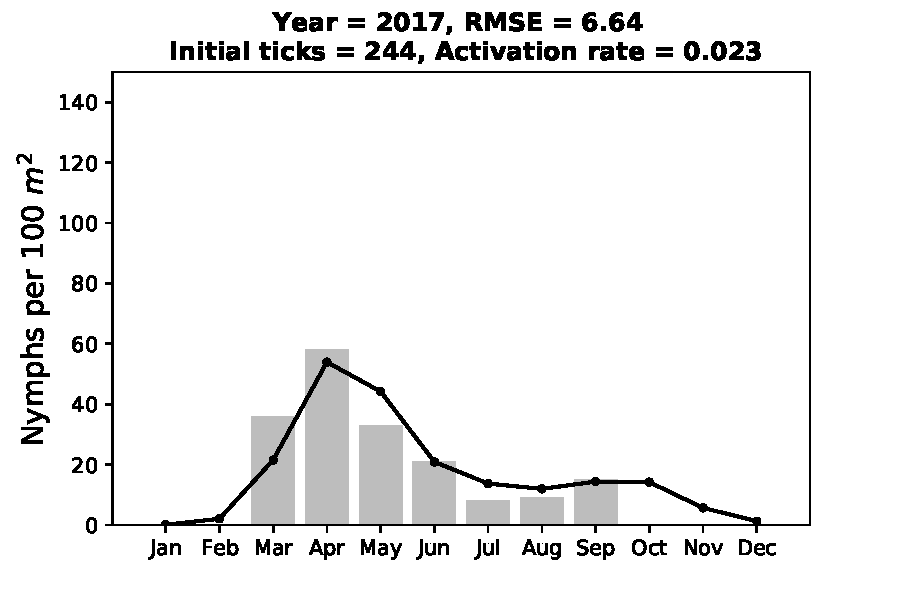
\includegraphics[width=\linewidth]{figures/s1/s1_2017}
\end{minipage}
\begin{minipage}[c]{0.40\linewidth}
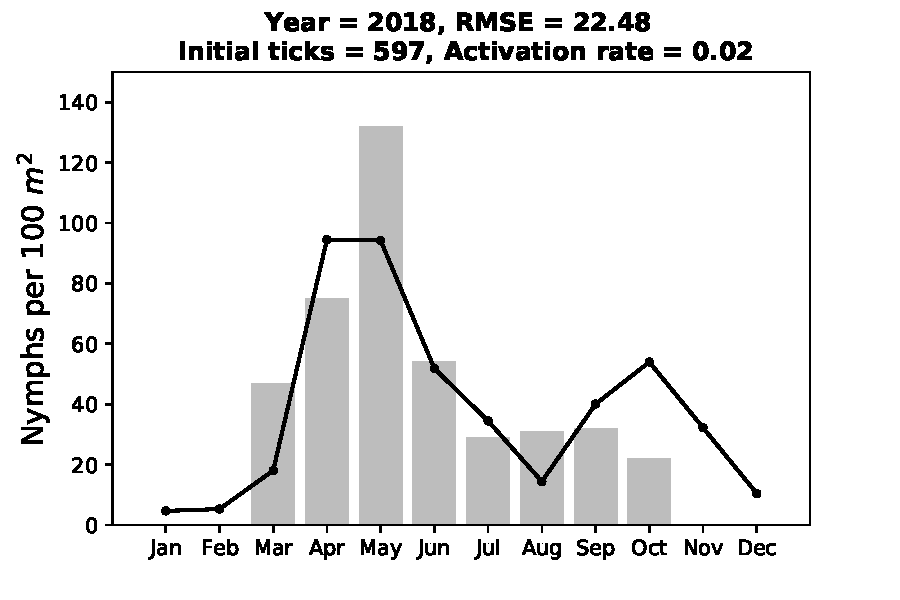
\includegraphics[width=\linewidth]{figures/s1/s1_2018}
\end{minipage}
\caption{Simulated and observed monthly nymphal densities (y-axis) for all 10 validation years (2009 - 2018) with minimal total RMSE of \textbf{sensitivity analysis S1}. The grey
bars represent the observed tick densities while the black line represents the simulated tick densities for each month of a year (x-axis). The activations rate $r_{opt} = 0.02$
minimises the total RMSE.}
\label{fig:initial_ticks_with_beech}
\end{figure}


\newpage
\subsection{S2: Equal number of larvae and nymphs with beech mast deactivated}
In this sensitivity analysis we use the same parameter variation as in the previous analysis. The only difference is that we have deactivated the beech mast in the model. The
initial values for larvae are therefore not adjusted in dependence of the beech mast fructification index at the beginning of the simulation run.

\begin{enumerate}
\item The initial number of nymphs was varied \underline{from} \textbf{1} \underline{to} \textbf{800} with a \underline{step size} of \textbf{1}.
\item The initial number of larvae was set to the initial number of nymphs.
\item The activation rate was varied \underline{from} \textbf{0.016} \underline{to} \textbf{0.022} with a \underline{step size} of \textbf{0.001}.
\end{enumerate}

When looking at the 3D scatterplots (see Figure\ref{fig:initial_ticks_without_beech_error}), it can immediately be seen that they look almost identical compared to the
scatterplots of the sensitivity analysis S1. Also here, the minimum RMSE values for each year are located within a narrow parameter range of initial ticks and there is no clear
effect of the activation rate $r$. A closer look reveals that some of the curves are slightly steeper and the level of some RMSE values is slightly higher than in sensitivity
analysis S1.

\begin{figure}[h!]
\centering
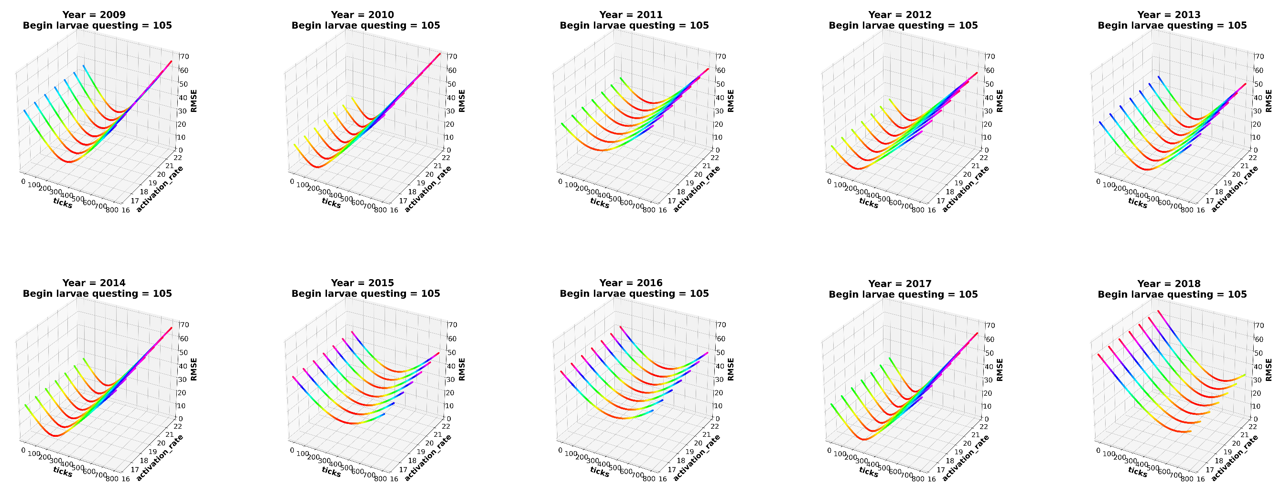
\includegraphics[width=\linewidth]{figures/initial_ticks_without_beech_error}
\caption{3D scatterplots of \textbf{sensitivity analysis S2} for all 10 validation years (2009 - 2018). Each of the plots is contrasting the initial number of larvae and nymphs
(labeled as \textit{ticks}) on the x-axis, the activation rate on the y-axis and the RMSE on the z-axis. The colour indicates how large the RMSE value is. Shades of red
represent low RMSE values and shades of yellow, green and purple represent higher RMSE values.}
\label{fig:initial_ticks_without_beech_error}
\end{figure}

The estimation of the optimal activation rate reveals a slightly higher value of $r_{opt} = 0.021$ compared to sensitivity analysis S1. The comparison of the simulated with
the observed data reveals only a few differences compared to sensitivity analysis S1 (see Figure~\ref{fig:initial_ticks_without_beech}). In particular, without beech mast the
second peak seems slightly stronger in some years (2009, 2010, 2012, 2014, 2015, 2016). In 2011, 2012, 2015 and 2018 the RMSE is slightly lower and in 2009, 2010, 2013, 2014
and 2016 the RMSE is higher compared to the sensitivity analysis with activated beech mast. In 2017 the RMSE has not changed. The overall qualitative patterns remains
the same. The sum of the RMSE values of the 10-year period is $RMSE_{total} = 154.89$. This value is higher than in S1 and indicates that the deactivation of the beech mast
worsens the matching with the observed data.

\begin{figure}[h!]
\centering
\begin{minipage}[c]{0.40\linewidth}
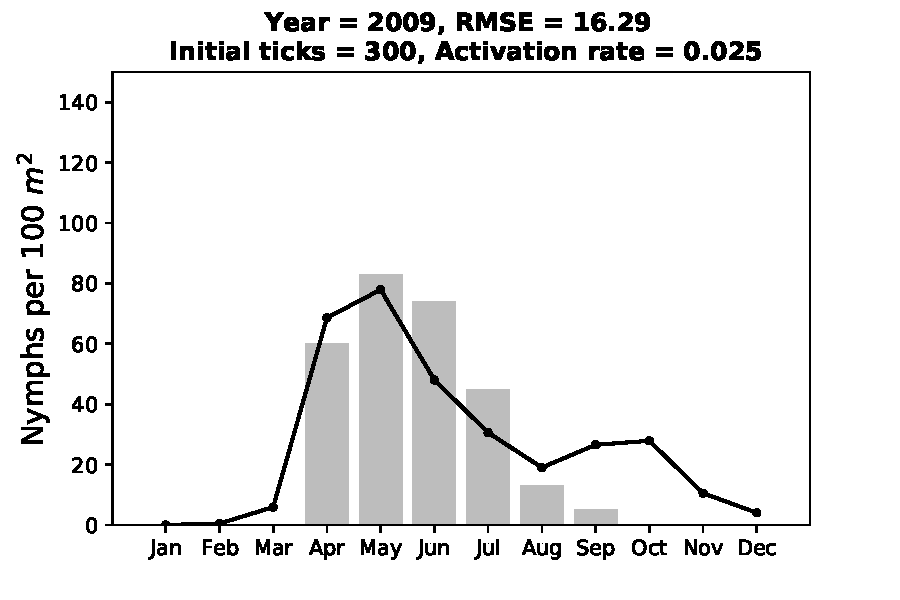
\includegraphics[width=\linewidth]{figures/s2/s2_2009}
\end{minipage}
\begin{minipage}[c]{0.40\linewidth}
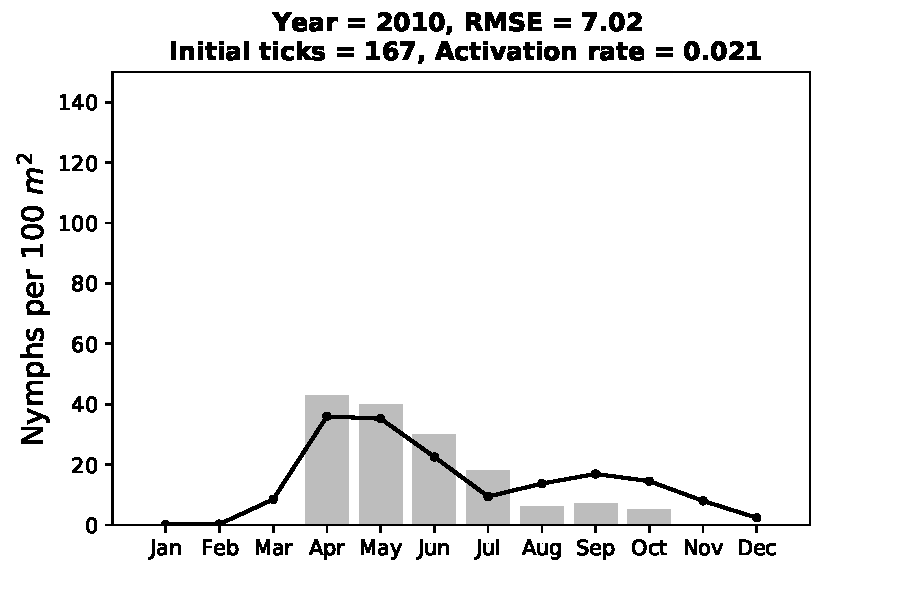
\includegraphics[width=\linewidth]{figures/s2/s2_2010}
\end{minipage}
\begin{minipage}[c]{0.40\linewidth}
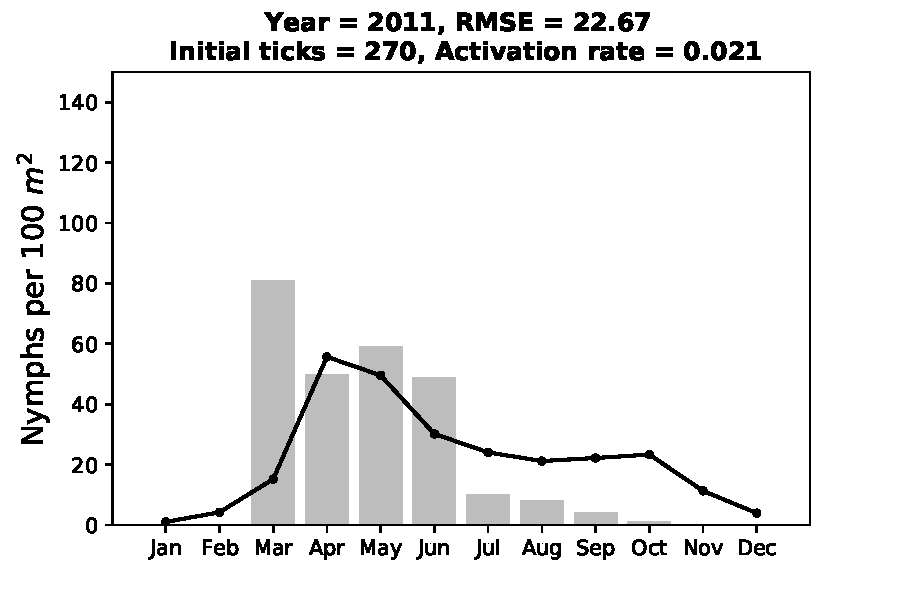
\includegraphics[width=\linewidth]{figures/s2/s2_2011}
\end{minipage}
\begin{minipage}[c]{0.40\linewidth}
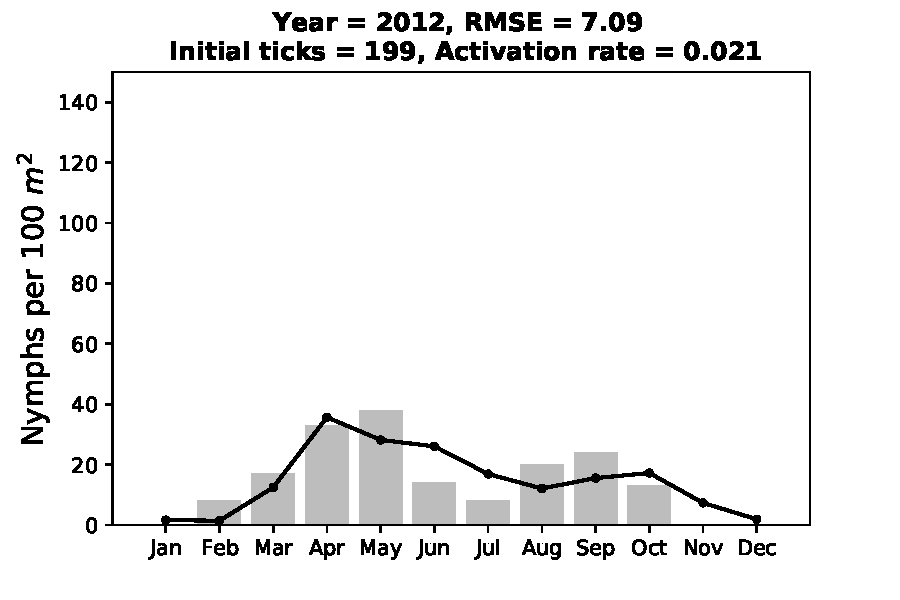
\includegraphics[width=\linewidth]{figures/s2/s2_2012}
\end{minipage}
\begin{minipage}[c]{0.40\linewidth}
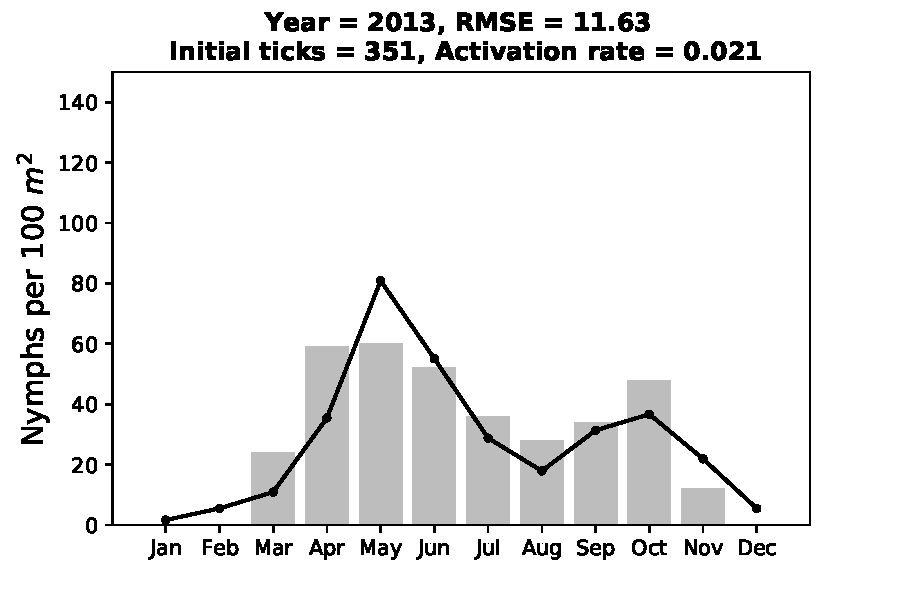
\includegraphics[width=\linewidth]{figures/s2/s2_2013}
\end{minipage}
\begin{minipage}[c]{0.40\linewidth}
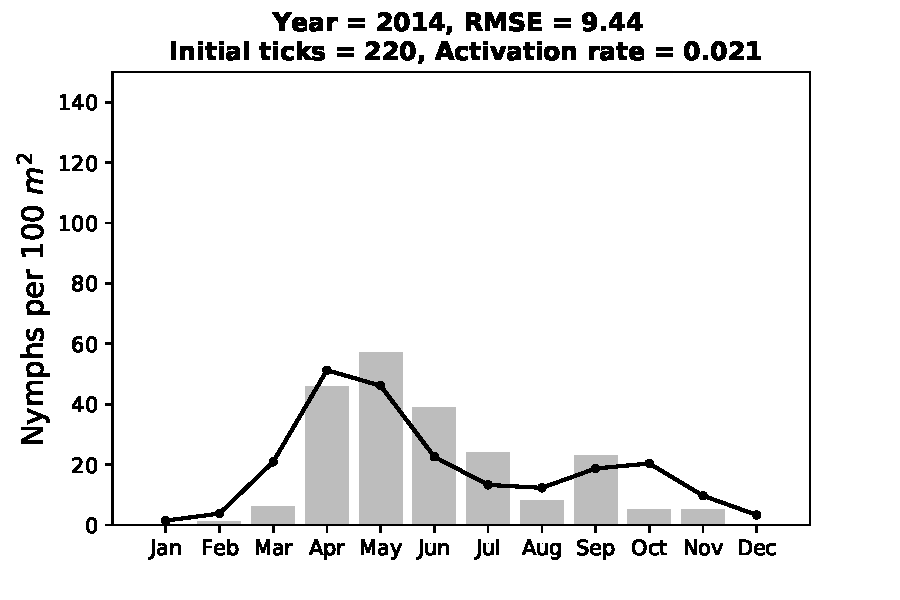
\includegraphics[width=\linewidth]{figures/s2/s2_2014}
\end{minipage}
\begin{minipage}[c]{0.40\linewidth}
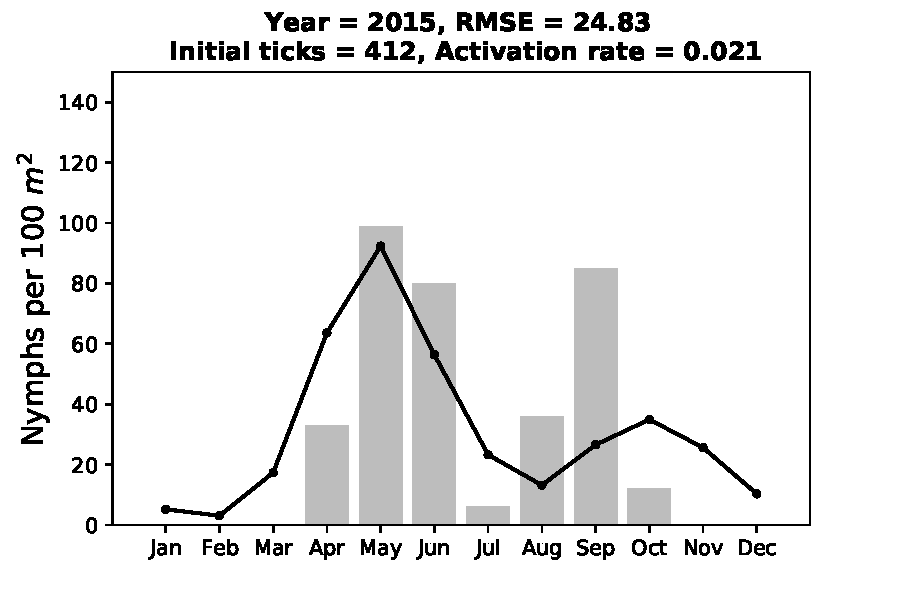
\includegraphics[width=\linewidth]{figures/s2/s2_2015}
\end{minipage}
\begin{minipage}[c]{0.40\linewidth}
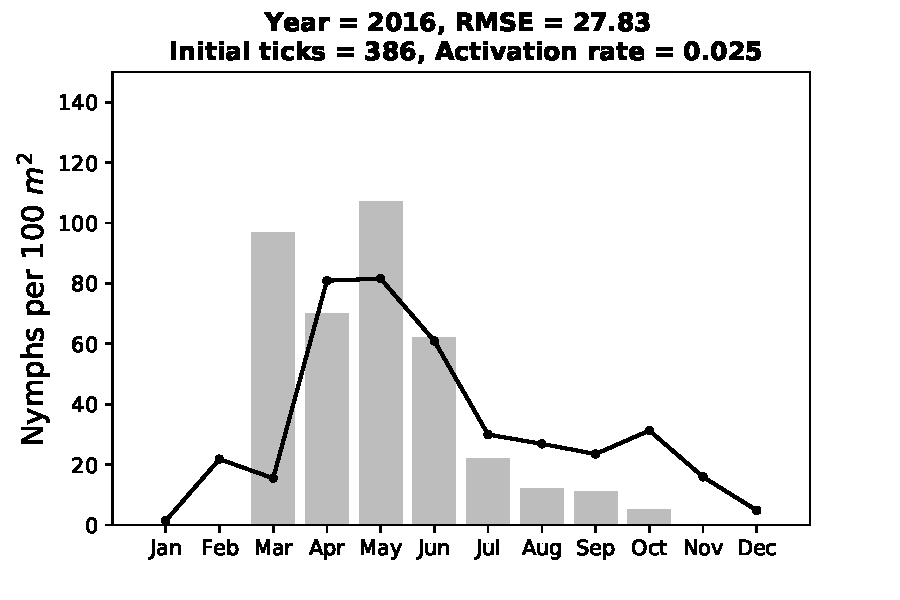
\includegraphics[width=\linewidth]{figures/s2/s2_2016}
\end{minipage}
\begin{minipage}[c]{0.40\linewidth}
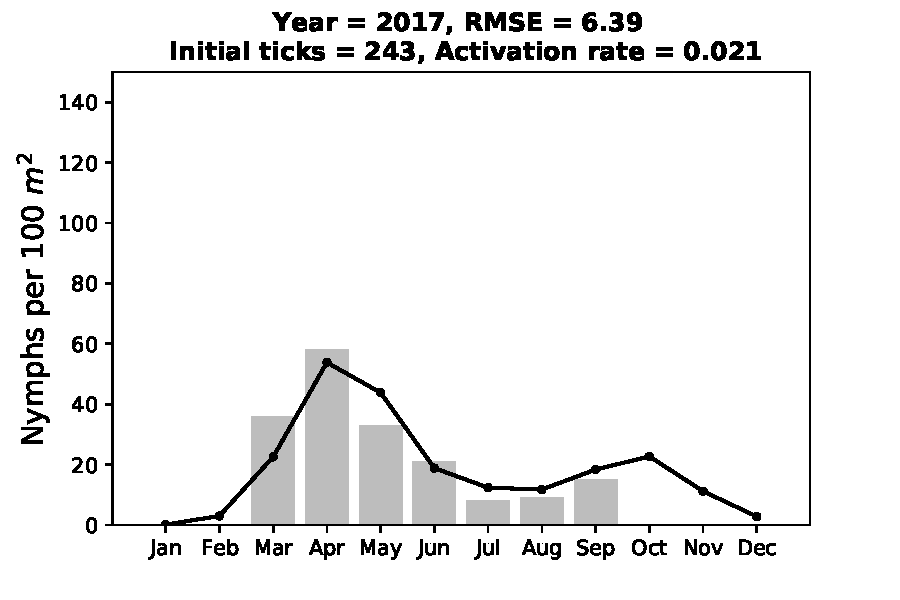
\includegraphics[width=\linewidth]{figures/s2/s2_2017}
\end{minipage}
\begin{minipage}[c]{0.40\linewidth}
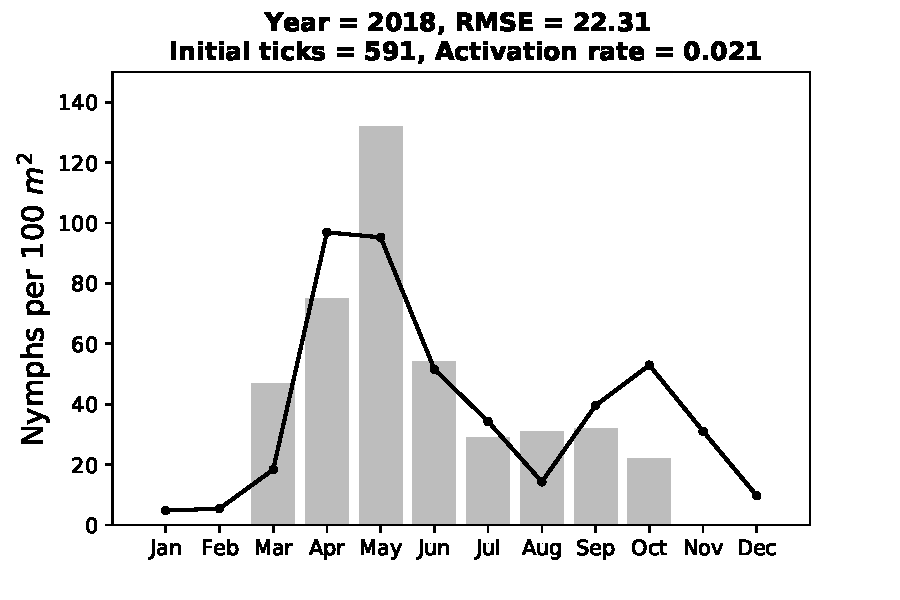
\includegraphics[width=\linewidth]{figures/s2/s2_2018}
\end{minipage}
\caption{Simulated and observed monthly nymphal densities (y-axis) for all 10 validation years (2009 - 2018) with minimal total RMSE of \textbf{sensitivity analysis S2}. The
grey bars represent the observed tick densities while the black line represents the simulated tick densities for each month of a year (x-axis). The activations rate of
$r_{opt}= 0.021$ minimises the total RMSE.}
\label{fig:initial_ticks_without_beech}
\end{figure}


\newpage
\subsection{S3: Larvae and nymphs individual variation, with beech mast activated}
In this sensitivity analysis we independently varied the initial number of larvae and nymphs and the activation rate $r$ in the following way:

\begin{enumerate}
\item The initial number of larvae was varied \underline{from} \textbf{0} \underline{to} \textbf{800} with a \underline{step size} of \textbf{10}.
\item The initial number of nymphs was varied \underline{from} \textbf{10} \underline{to} \textbf{800} with a \underline{step size} of \textbf{10}.
\item The activation rate was varied \underline{from} \textbf{0.016} \underline{to} \textbf{0.022} with a \underline{step size} of \textbf{0.001}.
\end{enumerate}

The 3D scatterplots of this sensitivity analysis are contrasting the initial number of larvae on the x-axis and the initial number of nymphs on the y-axis with the corresponding
RMSE value on the z-axis (see Figure~\ref{fig:independent_initial_ticks_with_beech_error}). The plots presented here show the results for the optimal activation rate
$r_{opt}= 0.02$. It is immediately apparent that the minimal RMSE values are located on a small strip whose position is defined by a narrow parameter range of initial nymphs on the
y-axis. Both higher and lower values would lead to an increase of the RMSE. Surprisingly, the initial number of larvae has little effect on the RMSE value. Only in the years
2009 and 2011 there is a clearly visible influence of the initial larvae. In these two years, the RMSE increases with an increasing number of initial larvae. Hence, the optimal
value is zero in each of the two years.
When comparing the simulated with the observed data (see Figure\ref{fig:independent_initial_ticks_with_beech}), it can be seen that the independent initialisation of larvae and
nymphs leads to a clear improvement of the overall RMSE with a value of $RMSE_{total} = 137.13$ (S1: 147.85, S2: 154.89). Although still not perfect, compared to the sensitivity
analyses S1 and S2, the second peak is clearly better captured. In particular, a second peak is no longer simulated by the model if no peak actually exists.

\begin{figure}[h!]
\centering
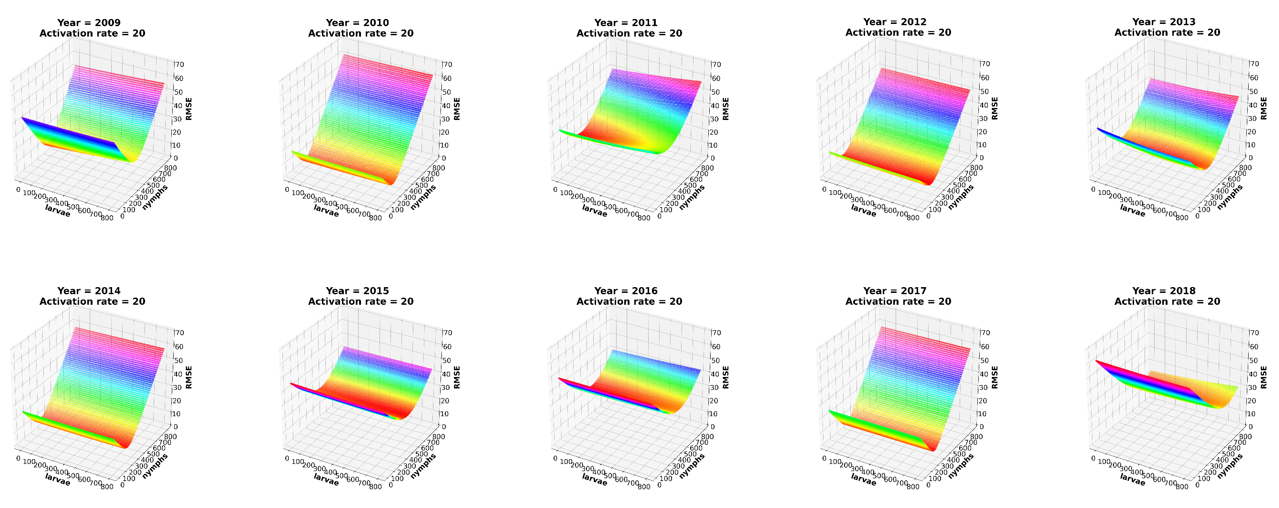
\includegraphics[width=\linewidth]{figures/independent_initial_ticks_with_beech_error}
\caption{3D scatterplots of \textbf{sensitivity analysis S3} for all 10 validation years (2009 - 2018). Each of the ten plots is contrasting the initial number of larvae on the
x-axis and the initial number of nymphs the y-axis with the corresponding RMSE value on the z-axis for the optimal activation rate $r_{opt} = 0.02$. The colour indicates how large
the RMSE value is. Shades of red represent low RMSE values and shades of yellow, green and purple represent higher RMSE values.}
\label{fig:independent_initial_ticks_with_beech_error}
\end{figure}

\begin{figure}[h!]
\centering
\begin{minipage}[c]{0.40\linewidth}
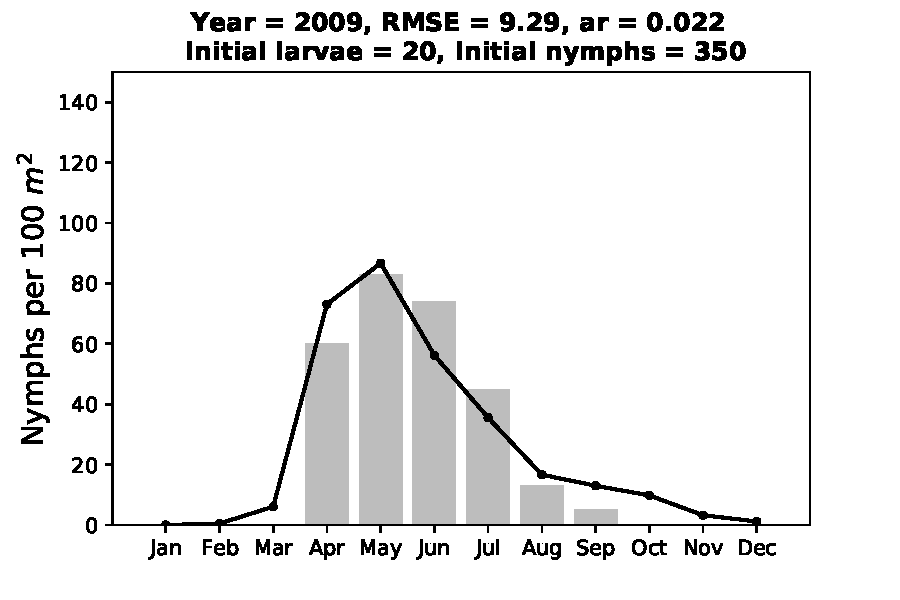
\includegraphics[width=\linewidth]{figures/s3/s3_2009}
\end{minipage}
\begin{minipage}[c]{0.40\linewidth}
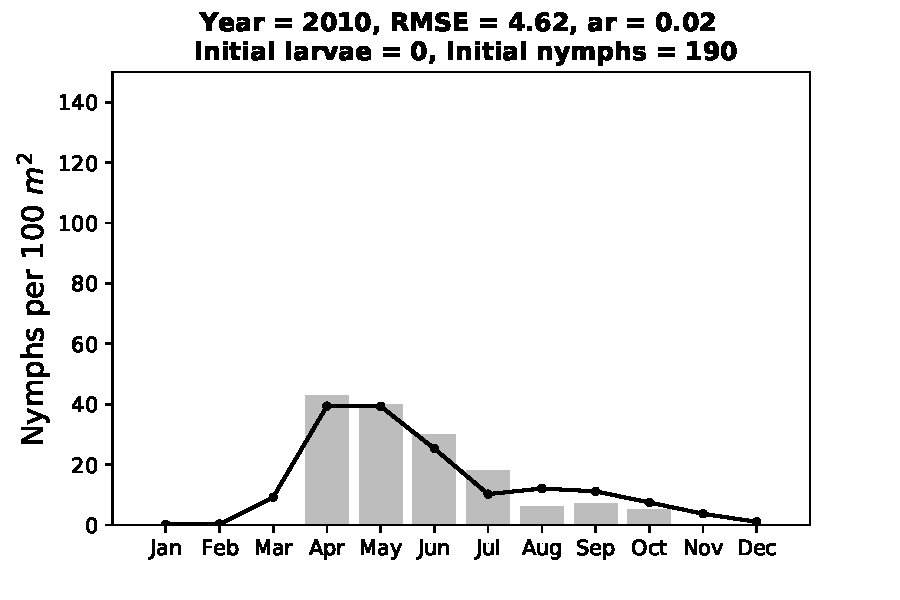
\includegraphics[width=\linewidth]{figures/s3/s3_2010}
\end{minipage}
\begin{minipage}[c]{0.40\linewidth}
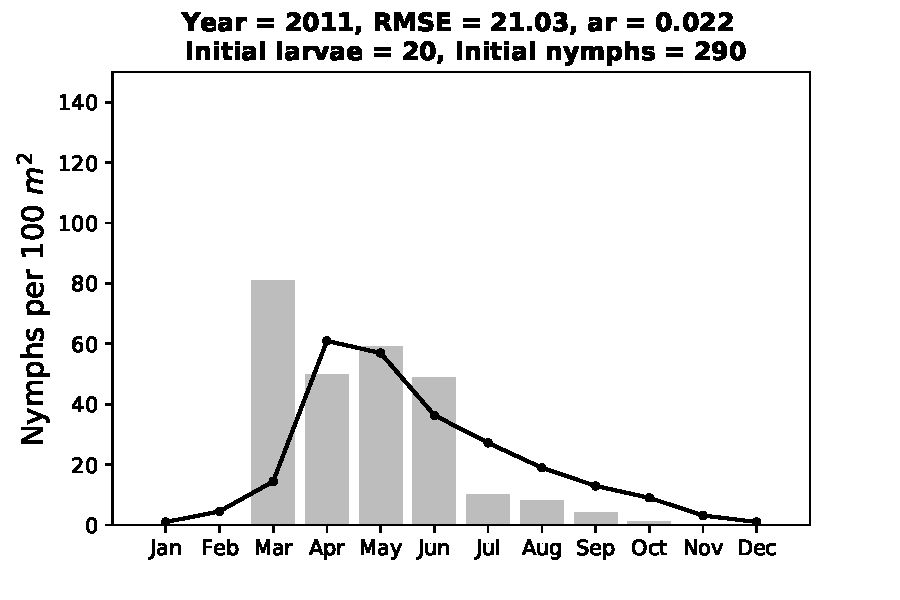
\includegraphics[width=\linewidth]{figures/s3/s3_2011}
\end{minipage}
\begin{minipage}[c]{0.40\linewidth}
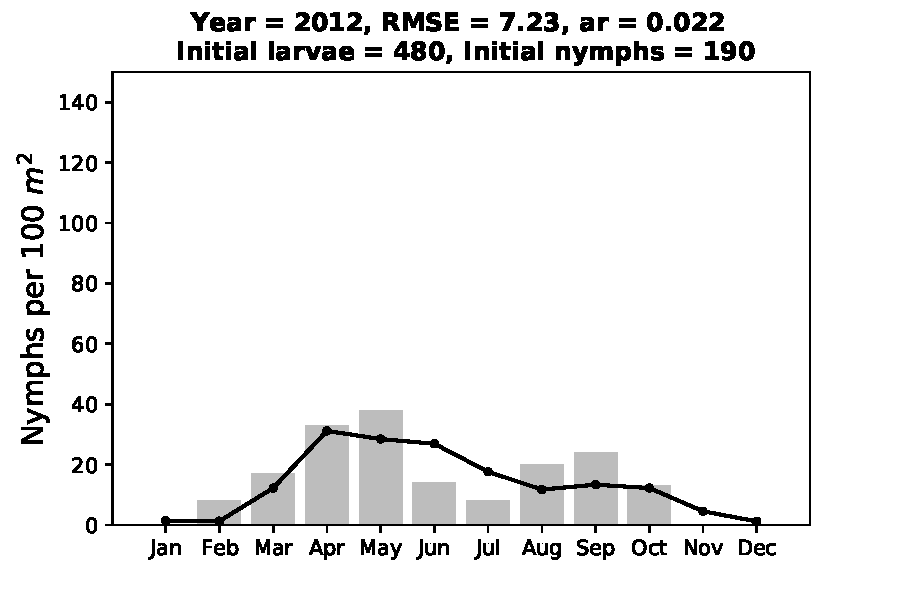
\includegraphics[width=\linewidth]{figures/s3/s3_2012}
\end{minipage}
\begin{minipage}[c]{0.40\linewidth}
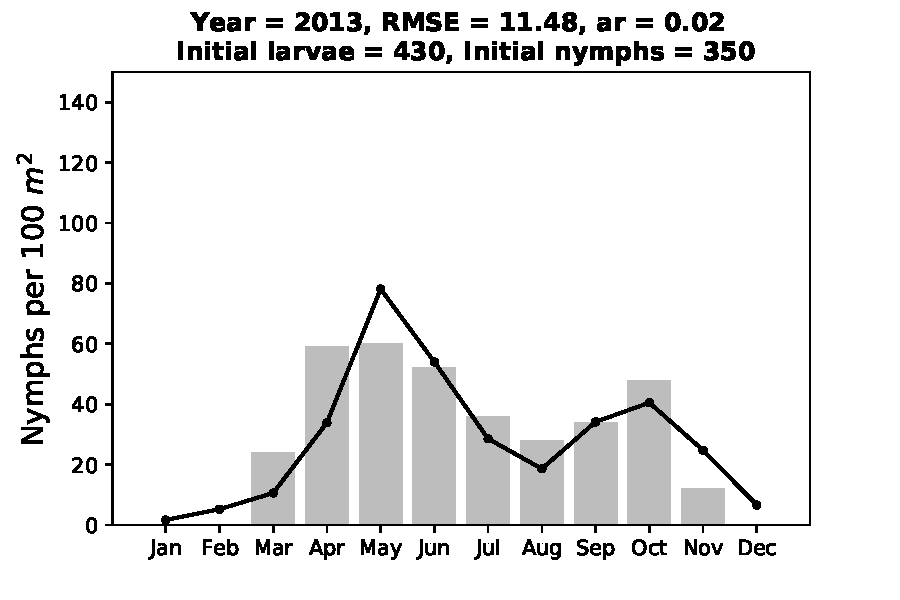
\includegraphics[width=\linewidth]{figures/s3/s3_2013}
\end{minipage}
\begin{minipage}[c]{0.40\linewidth}
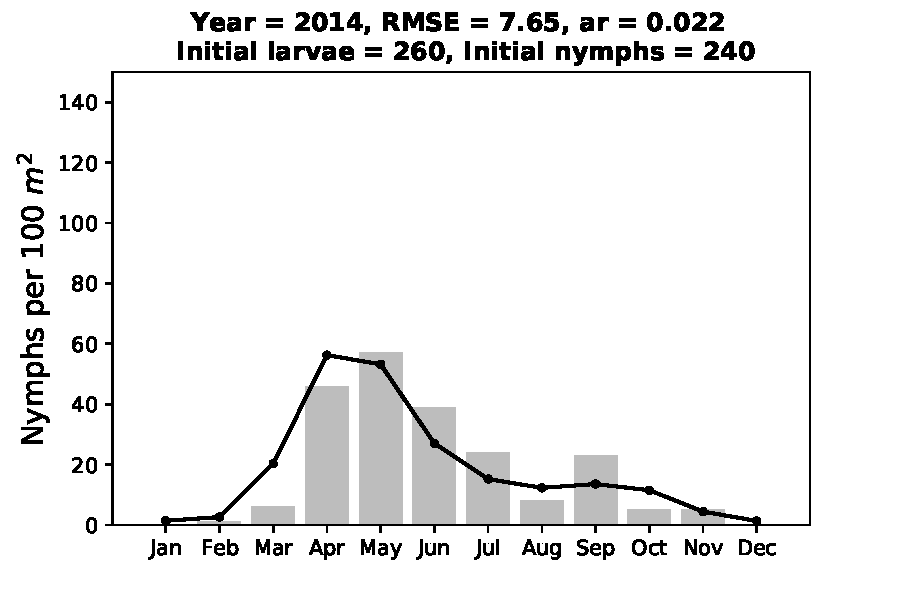
\includegraphics[width=\linewidth]{figures/s3/s3_2014}
\end{minipage}
\begin{minipage}[c]{0.40\linewidth}
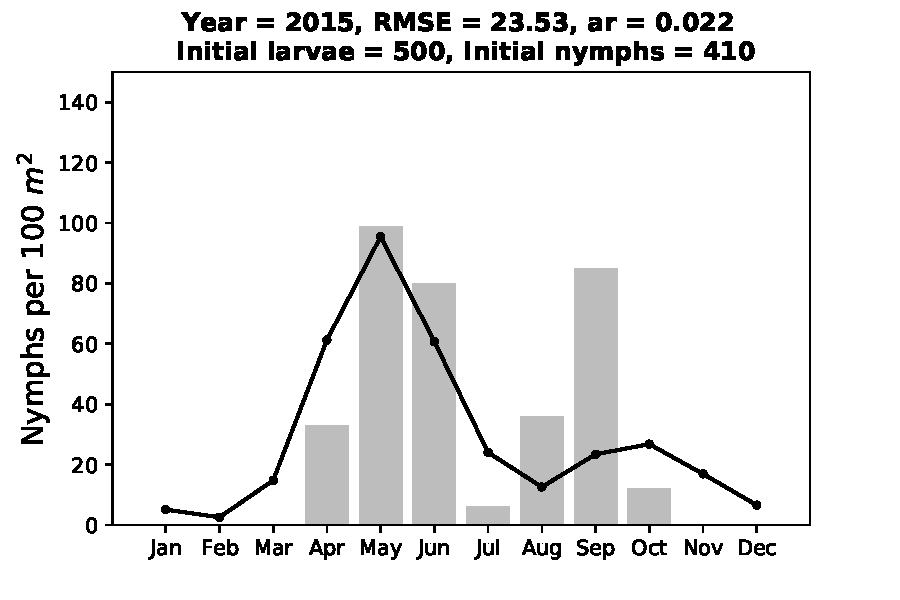
\includegraphics[width=\linewidth]{figures/s3/s3_2015}
\end{minipage}
\begin{minipage}[c]{0.40\linewidth}
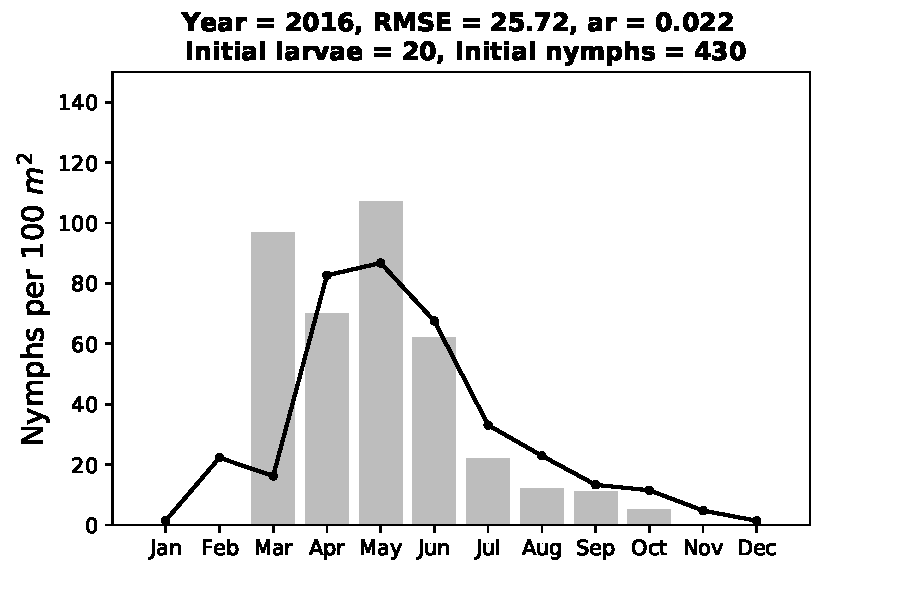
\includegraphics[width=\linewidth]{figures/s3/s3_2016}
\end{minipage}
\begin{minipage}[c]{0.40\linewidth}
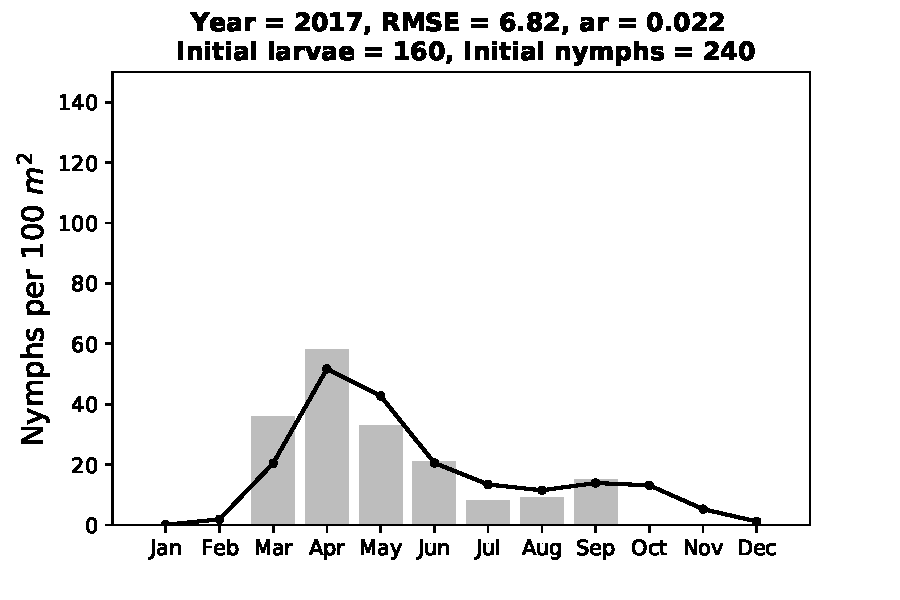
\includegraphics[width=\linewidth]{figures/s3/s3_2017}
\end{minipage}
\begin{minipage}[c]{0.40\linewidth}
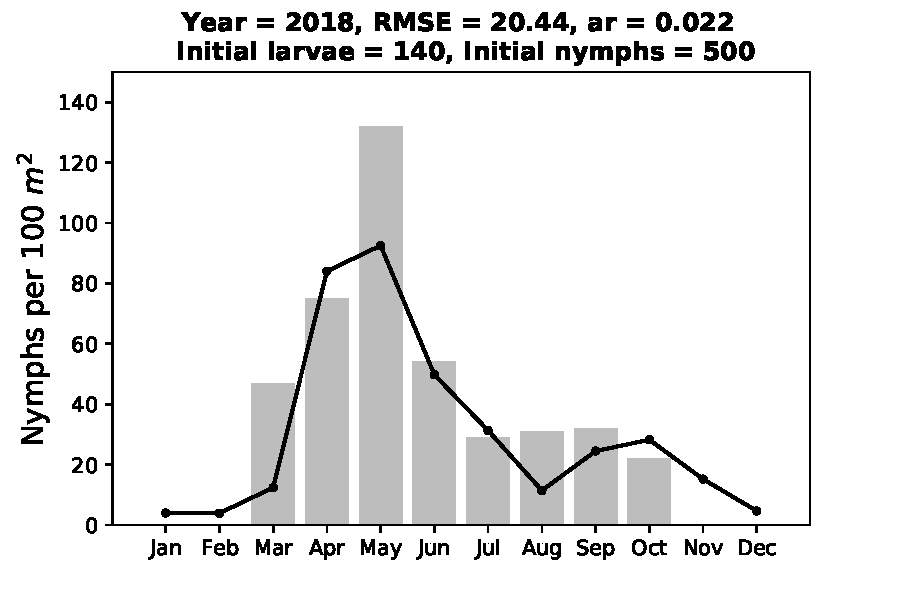
\includegraphics[width=\linewidth]{figures/s3/s3_2018}
\end{minipage}
\caption{Simulated and observed monthly nymphal densities (y-axis) for all 10 validation years (2009 - 2018) with minimal total RMSE of \textbf{sensitivity analysis S3}. The grey
bars represent the observed tick densities while the black line represents the simulated tick densities for each month of a year (x-axis). The activations rate of
$r_{opt}= 0.02$ minimises the total RMSE.}
\label{fig:independent_initial_ticks_with_beech}
\end{figure}


\newpage
\subsection{S4: Larvae and nymphs individual variation, with beech mast deactivated}
In this sensitivity analysis we independently varied the initial number of larvae and nymphs and the activation rate $r$ in the following way:

\begin{enumerate}
\item The initial number of larvae was varied \underline{from} \textbf{0} \underline{to} \textbf{800} with a \underline{step size} of \textbf{10}.
\item The initial number of nymphs was varied \underline{from} \textbf{10} \underline{to} \textbf{800} with a \underline{step size} of \textbf{10}.
\item The activation rate was varied \underline{from} \textbf{0.016} \underline{to} \textbf{0.022} with a \underline{step size} of \textbf{0.001}.
\end{enumerate}

With deactivated beech mast, the result of this sensitivity analysis are very similar compared to the results of the previous sensitivity analysis with activated beech mast.
The scatterplots (with optimal activation rate $r_{opt}= 0.02$) show that the initial number of larvae has a slightly larger effect on the RMSE value (see
Figure\ref{fig:independent_initial_ticks_without_beech_error}). Now there is also a gradient visible for the years 2010, 2012, 2014 and 2016, i.e.\ with increasing numbers of
initial larvae, the RMSE value also increases.

\begin{figure}[h!]
\centering
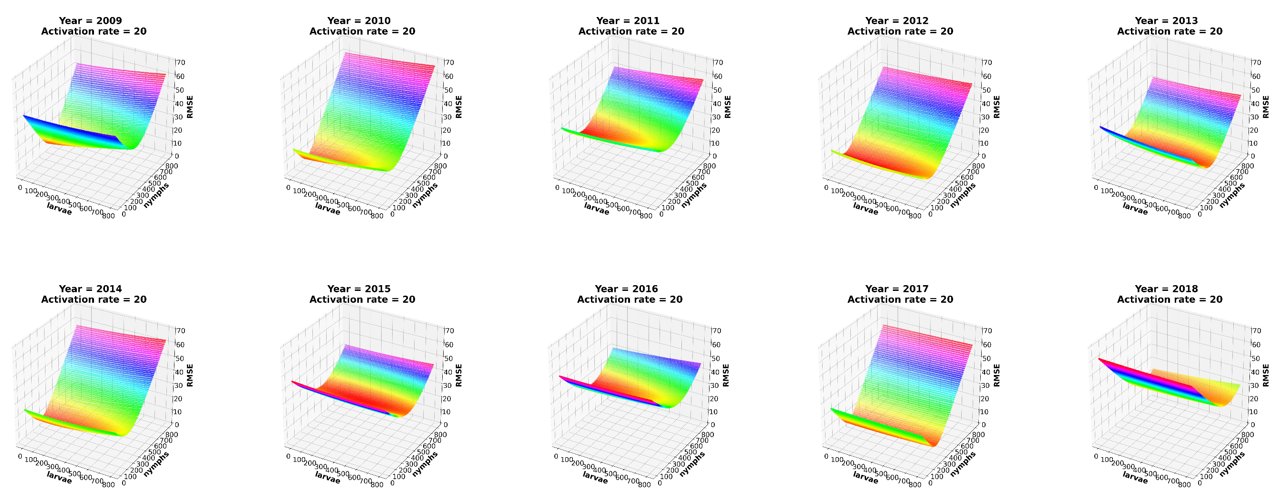
\includegraphics[width=\linewidth]{figures/independent_initial_ticks_without_beech_error}
\caption{3D scatterplots of \textbf{sensitivity analysis S4} for all 10 validation years (2009 - 2018). Each of the ten plots is contrasting the initial number of larvae on the
x-axis and the initial number of nymphs the y-axis with the corresponding RMSE value on the z-axis for the optimal activation rate $r_{opt} = 0.02$. The colour indicates how large
the RMSE value is. Shades of red represent low RMSE values and shades of yellow, green and purple represent higher RMSE values.}
\label{fig:independent_initial_ticks_without_beech_error}
\end{figure}

However, there are hardly any visible effects when comparing simulation and observation data (see Figure\ref{fig:independent_initial_ticks_without_beech}). Both the qualitaitve
pattern and the overall RMSE with $RMSE_{total} = 137.17$ are almost identical compared to sensitivity analyses S3. This suggests that if larvae and nymphs are
initialised independently, the model can just as well work without the beech mast module.

\begin{figure}[h!]
\centering
\begin{minipage}[c]{0.40\linewidth}
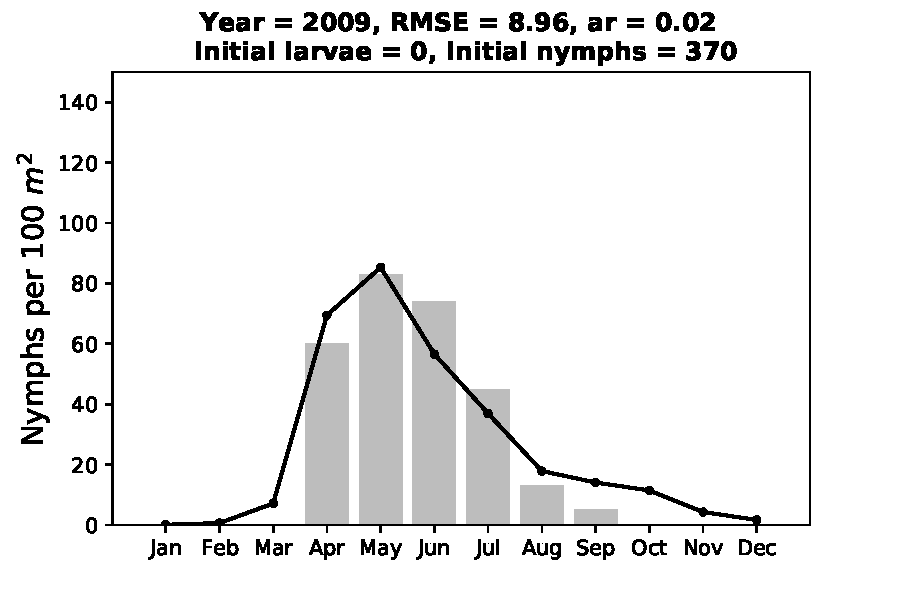
\includegraphics[width=\linewidth]{figures/s4/s4_2009}
\end{minipage}
\begin{minipage}[c]{0.40\linewidth}
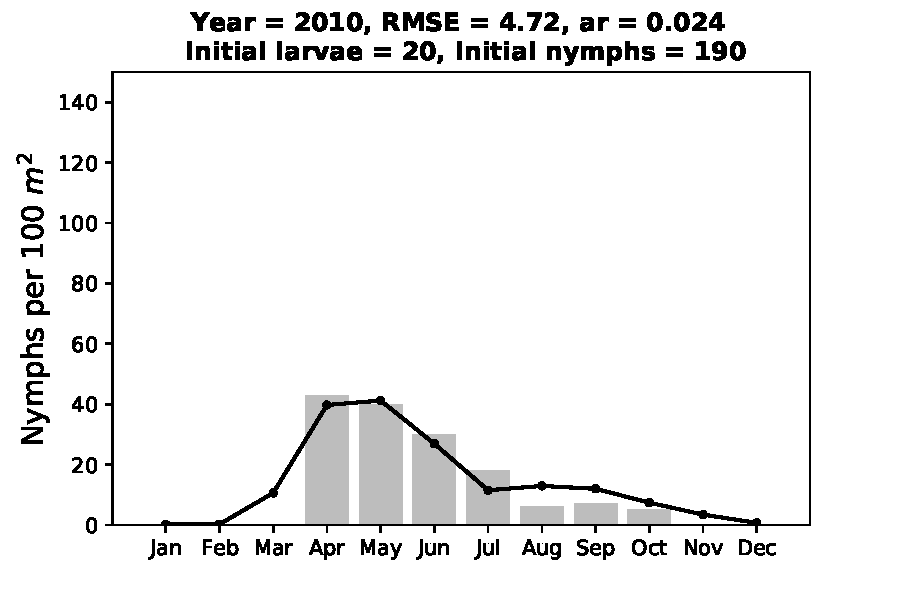
\includegraphics[width=\linewidth]{figures/s4/s4_2010}
\end{minipage}
\begin{minipage}[c]{0.40\linewidth}
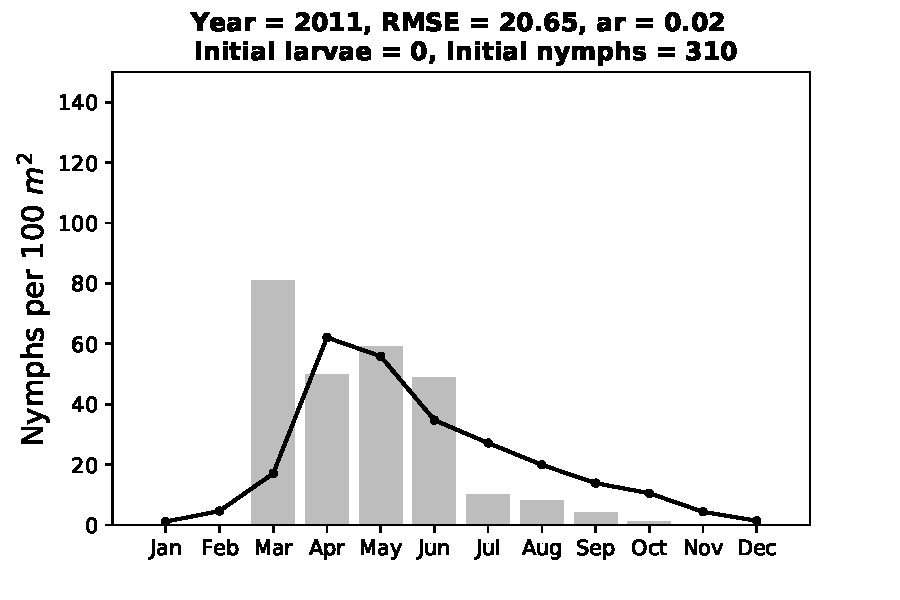
\includegraphics[width=\linewidth]{figures/s4/s4_2011}
\end{minipage}
\begin{minipage}[c]{0.40\linewidth}
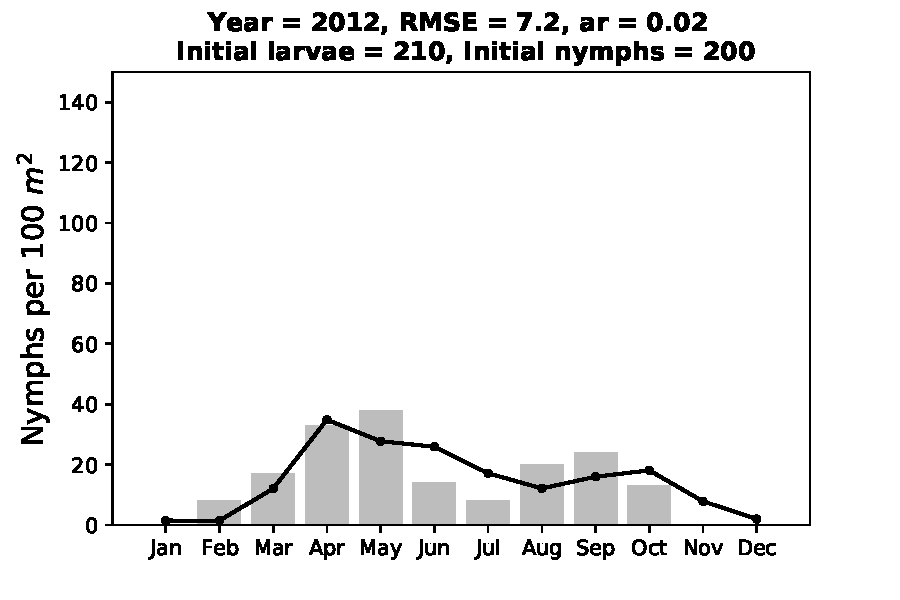
\includegraphics[width=\linewidth]{figures/s4/s4_2012}
\end{minipage}
\begin{minipage}[c]{0.40\linewidth}
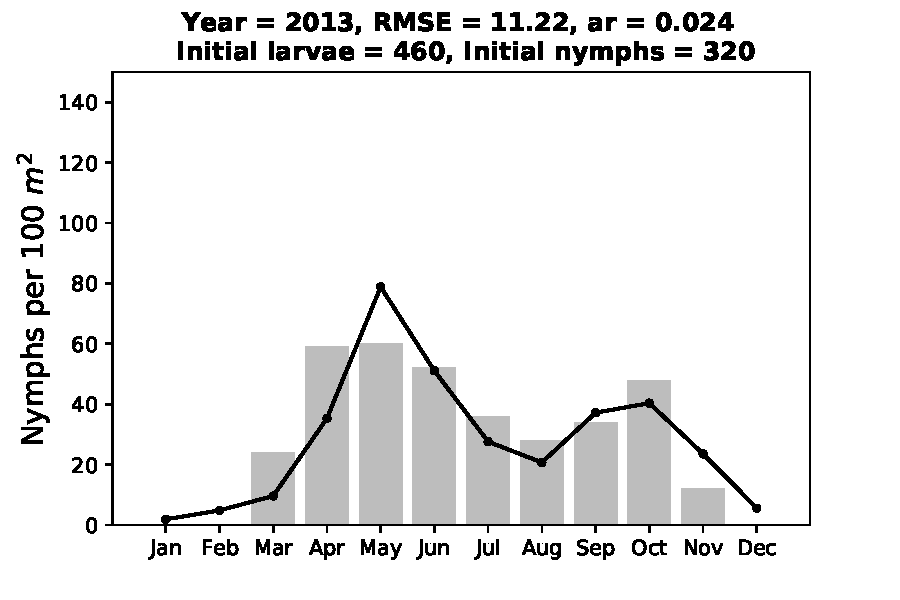
\includegraphics[width=\linewidth]{figures/s4/s4_2013}
\end{minipage}
\begin{minipage}[c]{0.40\linewidth}
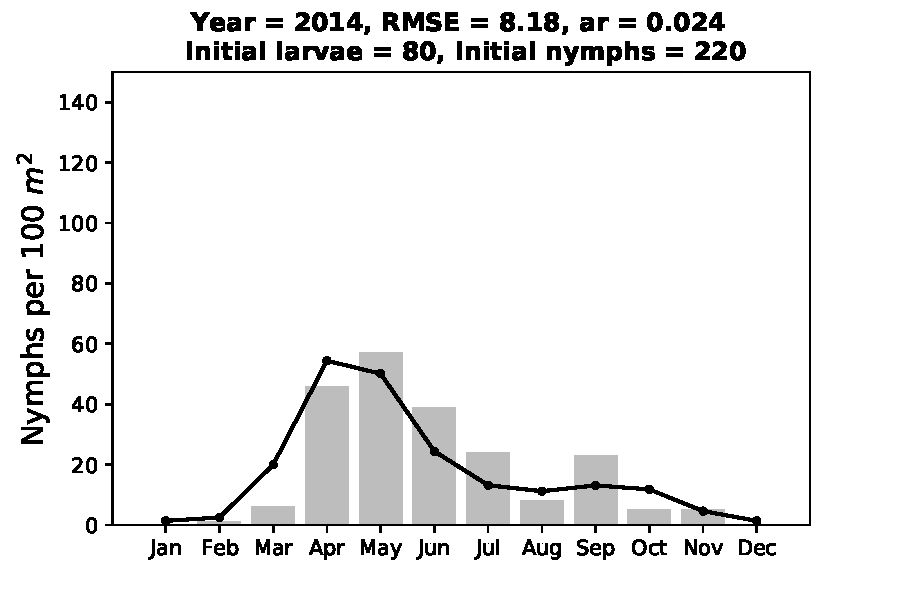
\includegraphics[width=\linewidth]{figures/s4/s4_2014}
\end{minipage}
\begin{minipage}[c]{0.40\linewidth}
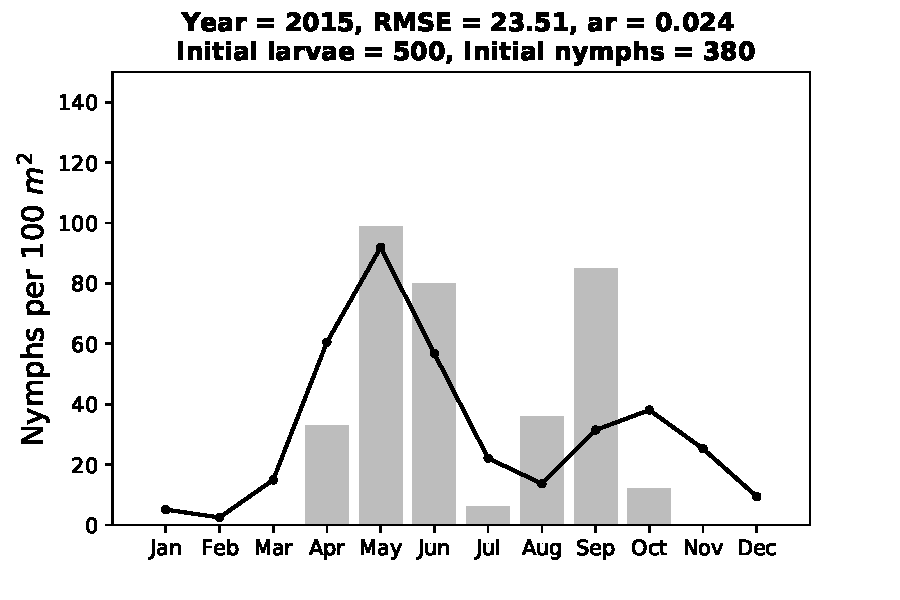
\includegraphics[width=\linewidth]{figures/s4/s4_2015}
\end{minipage}
\begin{minipage}[c]{0.40\linewidth}
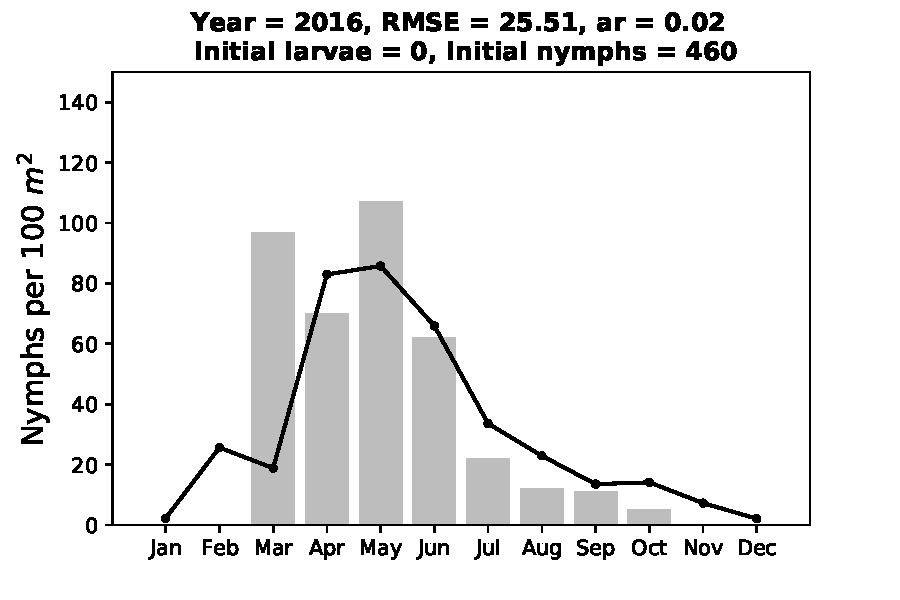
\includegraphics[width=\linewidth]{figures/s4/s4_2016}
\end{minipage}
\begin{minipage}[c]{0.40\linewidth}
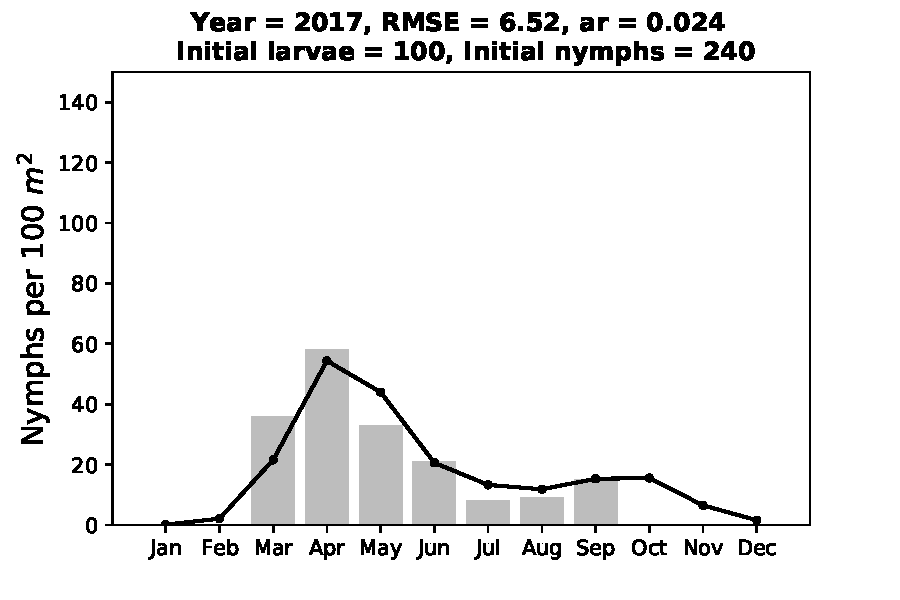
\includegraphics[width=\linewidth]{figures/s4/s4_2017}
\end{minipage}
\begin{minipage}[c]{0.40\linewidth}
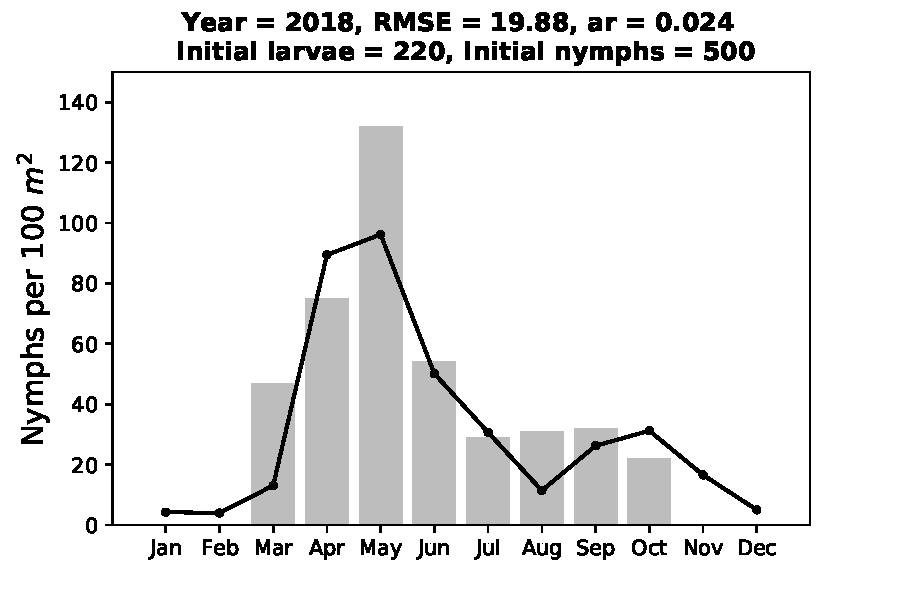
\includegraphics[width=\linewidth]{figures/s4/s4_2018}
\end{minipage}
\caption{Simulated and observed monthly nymphal densities (y-axis) for all 10 validation years (2009 - 2018) with minimal total RMSE of \textbf{sensitivity analysis S4}. The
grey bars represent the observed tick densities while the black line represents the simulated tick densities for each month of a year (x-axis). The activations rate
$r_{opt}= 0.02$ minimises the total RMSE.}
\label{fig:independent_initial_ticks_without_beech}
\end{figure}

\newpage
\subsection{S5: Higher share of initial number of Larvae, with beech mast activated}
In this sensitivity analysis, we wanted to illustrate the effect of a significantly higher number of initial larvae compared to initial nymphs on the second abundance peak.
Therefore, the following parameters were varied:

\begin{enumerate}
\item The initial number of nymphs was varied \underline{from} \textbf{0} \underline{to} \textbf{800} with a \underline{step size} of \textbf{10}.
\item The initial number of larvae was 4 $\times$ higher than the number of nymphs.
\item The activation rate was varied \underline{from} \textbf{0.016} \underline{to} \textbf{0.022} with a \underline{step size} of \textbf{0.001}.
\end{enumerate}

When looking directly at the graphs with the comparison to the observed data with an optimal activation rate of $r_{opt}= 0.021$ (see Figure\ref{fig:1nymphs_4larvae}), it is
noticeable that the second abundance peak appears very strongly in most years. Even if no peak activity was actually observed at the sampling site in Haselmühl, the model
simulates a relatively strong second peak. Not surprising, this goes hand in hand with a weak overall $RMSE_{total}$ of $192.13$.

\begin{figure}[h!]
\centering
\begin{minipage}[c]{0.40\linewidth}
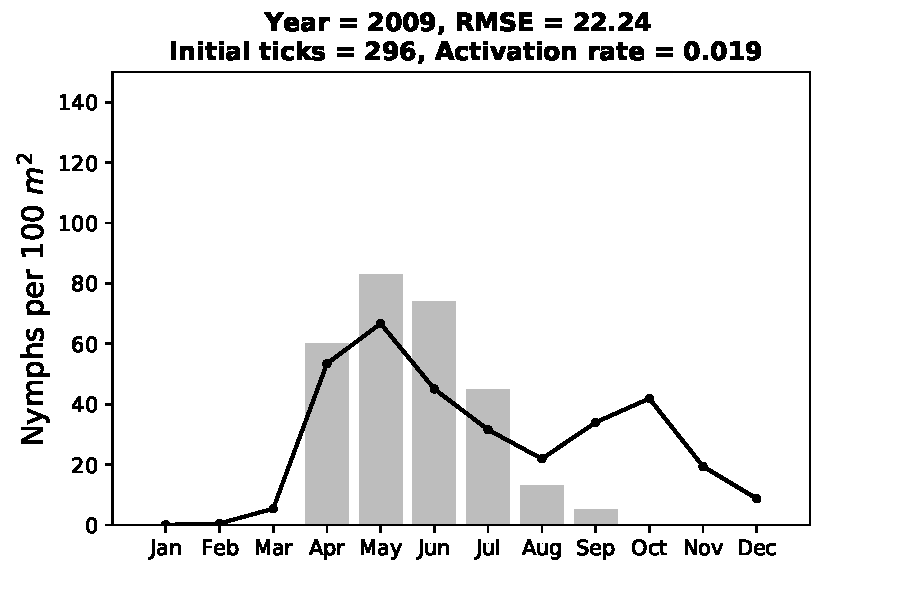
\includegraphics[width=\linewidth]{figures/s5/s5_2009}
\end{minipage}
\begin{minipage}[c]{0.40\linewidth}
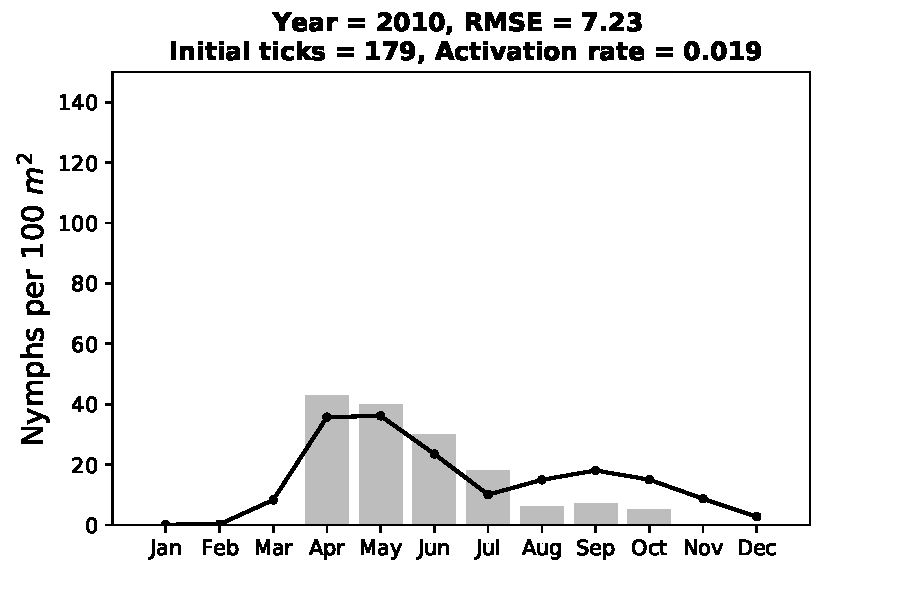
\includegraphics[width=\linewidth]{figures/s5/s5_2010}
\end{minipage}
\begin{minipage}[c]{0.40\linewidth}
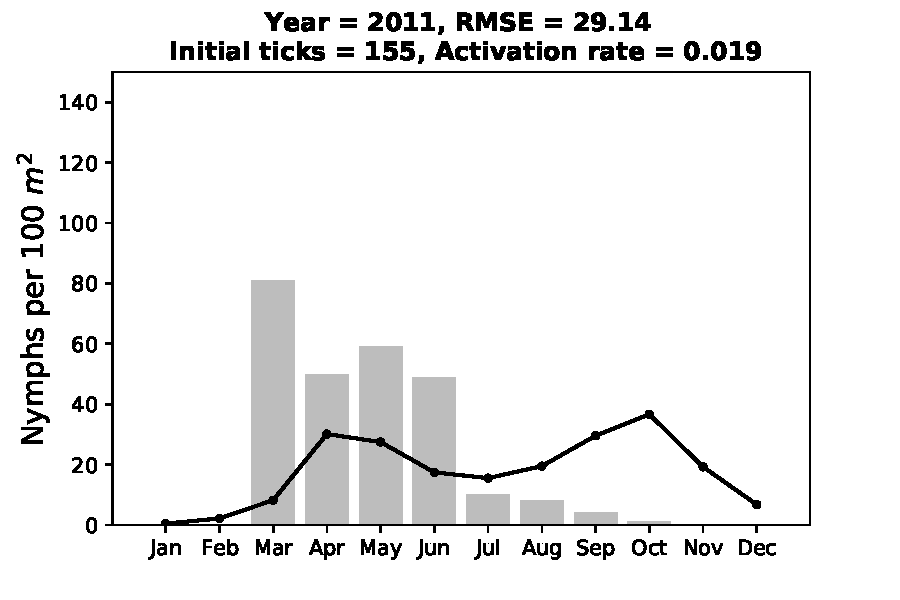
\includegraphics[width=\linewidth]{figures/s5/s5_2011}
\end{minipage}
\begin{minipage}[c]{0.40\linewidth}
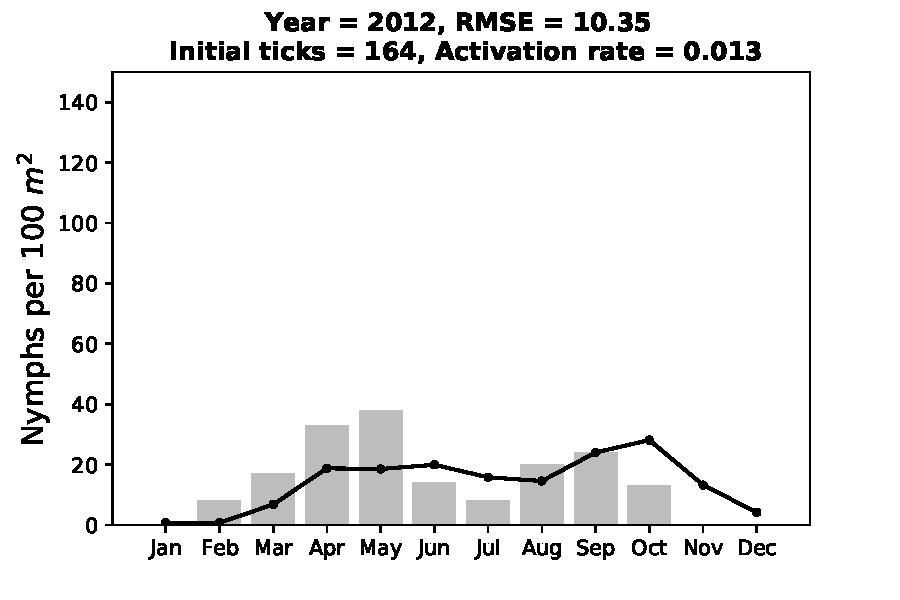
\includegraphics[width=\linewidth]{figures/s5/s5_2012}
\end{minipage}
\begin{minipage}[c]{0.40\linewidth}
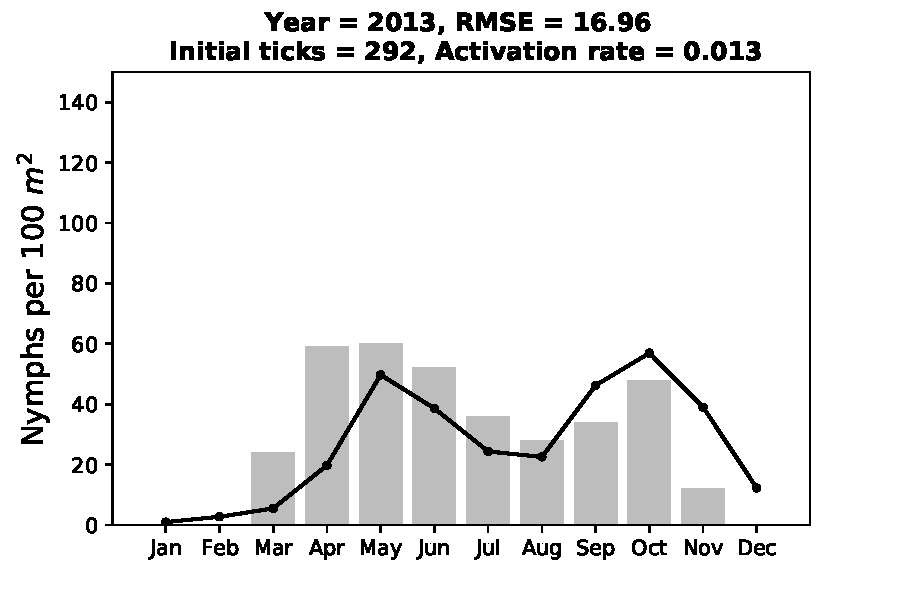
\includegraphics[width=\linewidth]{figures/s5/s5_2013}
\end{minipage}
\begin{minipage}[c]{0.40\linewidth}
\includegraphics[width=\linewidth]{figures/s5/s5_2014}
\end{minipage}
\begin{minipage}[c]{0.40\linewidth}
\includegraphics[width=\linewidth]{figures/s5/s5_2015}
\end{minipage}
\begin{minipage}[c]{0.40\linewidth}
\includegraphics[width=\linewidth]{figures/s5/s5_2016}
\end{minipage}
\begin{minipage}[c]{0.40\linewidth}
\includegraphics[width=\linewidth]{figures/s5/s5_2017}
\end{minipage}
\begin{minipage}[c]{0.40\linewidth}
\includegraphics[width=\linewidth]{figures/s5/s5_2018}
\end{minipage}
\caption{Simulated and observed monthly nymphal densities (y-axis) for all 10 validation years (2009 - 2018) with minimal total RMSE of \textbf{sensitivity analysis S5}. The
grey bars represent the observed tick densities while the black line represents the simulated tick densities for each month of a year (x-axis). The activations rate
$r_{opt}= 0.019$ minimises the total RMSE.}
\label{fig:1nymphs_4larvae}
\end{figure}


\section{Lessons Learned}
In summary we have learned from the model validation that

\begin{enumerate}
\item the IRIS simulation model captures the observed monthly nymphal densities overall relatively well in qualitative terms with some years performing worse and other years
performing better with regard to the RMSE value.
\item the first abundance peak of a given year simulated by the model matches the observation data relatively well in almost all years (exception: March 2011 and 2016).
\item under sensitivity analyses S1 and S2 (i.e.\ initialisation with equal numbers of initial larvae and nymphs) the second abundance peak of a given year was not always
captured well by the model. In many cases a second peak was modelled although no peak actually exists. However, under sensitivity analyses S2 and S3 (i.e.\ initialisation with
independent numbers of initial larvae and nymphs) performed much better in modelling the second peak.
\item the best matching (in terms of the overall RMSE) with the observed data was achieved when the optimal activation rate was approximately $r_{opt} = 0.02$ (1x 0.019,  3x 0
.02,  1x 0.021).
\item the initial number of larvae had only a very minor influence on the RMSE when the initial number of larvae and nymphs were varied independently (S3, S4).
\item with individual variation of initial larvae and nymphs (S3, S4), the influence of the beech mast had little effect.
\item the overall RMSE of the sensitivity analysis with equal numbers of initial larvae and nymphs was improved by the beech mast (S1, S2).
\item a strong increase of initial larvae led to an increase of the second abundance peak, but worsened the overall matching with observed data (S5).
\end{enumerate}

Table~\ref{tab:summary} shows the overall RMSE values and the optimal activations rates for all sensitivity analyses presented in this report.

\begin{table}[h!]
\caption{Summary of sensitivity analysis}
\label{tab:summary}
\begin{tabularx}{\textwidth}{lcc}
\toprule
\textbf{Sensitivity Analysis} & \textbf{$RMSE_{total}$} & \textbf{Optimal activation rate $r_{opt}$} \\
\midrule
S1 & 147.85 & 0.02 \\
S2 & 154.89 & 0.021 \\
S3 & 137.13 & 0.02 \\
S4 & 137.17 & 0.02 \\
S5 & 192.13 & 0.019 \\
\bottomrule
\end{tabularx}
\end{table}



\printbibliography[heading = bibintoc, title = {Bibliography}]

\clearpage

\begin{sidewaysfigure}[h!]
\centering
\includegraphics[width=\linewidth]{figures/initial_ticks_with_beech_error_v1.png}
\caption{3D scatterplots of \textbf{sensitivity analysis S1} for all 10 validation years (2009 - 2018). Each of the plots is contrasting the initial number of larvae and nymphs
(labeled as \textit{ticks}) on the x-axis, the activation rate on the y-axis and the RMSE on the z-axis. The colour indicates how large the RMSE value is. Shades of
red represent low RMSE values and shades of yellow, green and purple represent higher RMSE values.}
\label{fig:initial_ticks_with_beech_error_v1_roteted}
\end{sidewaysfigure}

\begin{sidewaysfigure}[h!]
\centering
\includegraphics[width=\linewidth]{figures/initial_ticks_with_beech_error.png}
\caption{3D scatterplots of \textbf{sensitivity analysis S1} for all 10 validation years (2009 - 2018). Each of the plots is contrasting the initial number of larvae and nymphs
(labeled as \textit{ticks}) on the x-axis, the activation rate on the y-axis and the RMSE on the z-axis. The colour indicates how large the RMSE value is. Shades of
red represent low RMSE values and shades of yellow, green and purple represent higher RMSE values.}
\label{fig:initial_ticks_with_beech_error_rotated}
\end{sidewaysfigure}

\begin{sidewaysfigure}[h!]
\centering
\includegraphics[width=\linewidth]{figures/initial_ticks_without_beech_error.png}
\caption{3D scatterplots of \textbf{sensitivity analysis S2} for all 10 validation years (2009 - 2018). Each of the plots is contrasting the initial number of larvae and nymphs
(labeled as \textit{ticks}) on the x-axis, the activation rate on the y-axis and the RMSE on the z-axis. The colour indicates how large the RMSE value is. Shades of red
represent low RMSE values and shades of yellow, green and purple represent higher RMSE values.}
\label{fig:initial_ticks_without_beech_error_rotated}
\end{sidewaysfigure}

\begin{sidewaysfigure}[h!]
\centering
\includegraphics[width=\linewidth]{figures/independent_initial_ticks_with_beech_error.png}
\caption{3D scatterplots of \textbf{sensitivity analysis S3} for all 10 validation years (2009 - 2018). Each of the ten plots is contrasting the initial number of larvae on the
x-axis and the initial number of nymphs the y-axis with the corresponding RMSE value on the z-axis for the optimal activation rate $r_{opt} = 0.02$. The colour indicates how large
the RMSE value is. Shades of red represent low RMSE values and shades of yellow, green and purple represent higher RMSE values.}
\label{fig:independent_initial_ticks_with_beech_error_rotated}
\end{sidewaysfigure}

\begin{sidewaysfigure}[h!]
\centering
\includegraphics[width=\linewidth]{figures/independent_initial_ticks_without_beech_error.png}
\caption{3D scatterplots of \textbf{sensitivity analysis S4} for all 10 validation years (2009 - 2018). Each of the ten plots is contrasting the initial number of larvae on the
x-axis and the initial number of nymphs the y-axis with the corresponding RMSE value on the z-axis for the optimal activation rate $r_{opt} = 0.02$. The colour indicates how large
the RMSE value is. Shades of red represent low RMSE values and shades of yellow, green and purple represent higher RMSE values.}
\label{fig:independent_initial_ticks_without_beech_error_rotated}
\end{sidewaysfigure}

\end{document}